%===============================================================================
% LaTeX sjabloon voor de bachelorproef toegepaste informatica aan HOGENT
% Meer info op https://github.com/HoGentTIN/latex-hogent-report
%===============================================================================

\documentclass[dutch,dit,thesis]{hogentreport}
\usepackage{lipsum} % For blind text, can be removed after adding actual content

\usepackage{graphicx}
\usepackage{caption}
\usepackage{subcaption}
\usepackage{float}


%% Pictures to include in the text can be put in the graphics/ folder
\graphicspath{{../graphics/}}

%% For source code highlighting, requires pygments to be installed
%% Compile with the -shell-escape flag!
%%\usepackage[chapter]{minted}
%% If you compile with the make_thesis.{bat,sh} script, use the following
%% import instead:
\usepackage{minted}

\usemintedstyle{solarized-light}

%% Formatting for minted environments.
\setminted{%
    autogobble,
    frame=lines,
    breaklines,
    linenos,
    tabsize=4
}

% Ensure the list of listings is in the table of contents



% Other packages not already included can be imported here

%%---------- Document metadata -------------------------------------------------
% TODO: Replace this with your own information
\author{Tariq Asifi}
\supervisor{Dhr. L. Smits}
\cosupervisor{Dhr. S. Boussemaere}
\title{De impact van simulatie- en emulatietools op netwerkvaardigheden in het hoger onderwijs: een vergelijkende analyse van GNS3 en Packet Tracer}
\academicyear{\advance\year by -1 \the\year--\advance\year by 1 \the\year}
\examperiod{1}
\degreesought{\IfLanguageName{dutch}{Professionele bachelor in de toegepaste informatica}{Bachelor of applied computer science}}
\partialthesis{false} %% To display 'in partial fulfilment'
%\institution{Internshipcompany BVBA.}

%% Add global exceptions to the hyphenation here
\hyphenation{back-slash}

%% The bibliography (style and settings are  found in hogentthesis.cls)
\addbibresource{bachproef.bib}            %% Bibliography file
\addbibresource{../voorstel/voorstel.bib} %% Bibliography research proposal
\defbibheading{bibempty}{}

%% Prevent empty pages for right-handed chapter starts in twoside mode
\renewcommand{\cleardoublepage}{\clearpage}

\renewcommand{\arraystretch}{1.2}

%% Content starts here.
\begin{document}

%---------- Front matter -------------------------------------------------------

\frontmatter

\hypersetup{pageanchor=false} %% Disable page numbering references
%% Render a Dutch outer title page if the main language is English
\IfLanguageName{english}{%
    %% If necessary, information can be changed here
    \degreesought{Professionele Bachelor toegepaste informatica}%
    \begin{otherlanguage}{dutch}%
       \maketitle%
    \end{otherlanguage}%
}{}

%% Generates title page content
\maketitle
\hypersetup{pageanchor=true}

%%=============================================================================
%% Voorwoord
%%=============================================================================

\chapter*{\IfLanguageName{dutch}{Woord vooraf}{Preface}}%
\label{ch:voorwoord}

%% TODO:
%% Het voorwoord is het enige deel van de bachelorproef waar je vanuit je
%% eigen standpunt (``ik-vorm'') mag schrijven. Je kan hier bv. motiveren
%% waarom jij het onderwerp wil bespreken.
%% Vergeet ook niet te bedanken wie je geholpen/gesteund/... heeft

Deze bachelorproef werd geschreven in het kader van het behalen van het diploma Bachelor in de Toegepaste Informatica, afstudeerrichting Systeem- en Netwerkbeheer. Tijdens het traject werd het oorspronkelijke onderzoeksonderwerp herzien. Na overleg met mijn promotor werd duidelijk dat het oorspronkelijke onderwerp onvoldoende aansloot bij de praktische haalbaarheid en academische relevantie. Daarom werd in samenspraak besloten om het onderzoek te verleggen naar een vergelijkende studie tussen Cisco Packet Tracer en GNS3. Dit nieuwe onderzoek sluit beter aan bij mijn opleiding, persoonlijke interesse en de beschikbare middelen, en vormde het uitgangspunt voor de bachelorproef die hier wordt uitgewerkt.

\vspace{0.3cm}

Dit eindwerk had ik niet kunnen realiseren zonder de steun en inzet van een aantal mensen, aan wie ik mijn oprechte dank wil uitspreken.

\vspace{0.3cm}

Mijn bijzondere dank gaat uit naar mijn promotor, de heer Lieven Smits. Zijn begeleiding, feedback en waardevolle adviezen hebben me geholpen om tot een sterk en relevant onderzoeksvoorstel te komen. Vooral tijdens de overgang naar een nieuw onderwerp heeft zijn bijdrage een belangrijke rol gespeeld in de goede afronding van deze bachelorproef.

\vspace{0.3cm}

Mijn dank gaat ook uit naar mijn copromotor, de heer Stijn Boussemaere, die bereid was het nieuwe onderwerp mee te ondersteunen. Zijn openheid, flexibiliteit en feedback hebben een belangrijke bijdrage geleverd aan het slagen van deze bachelorproef.
%%=============================================================================
%% Samenvatting
%%=============================================================================

% TODO: De "abstract" of samenvatting is een kernachtige (~ 1 blz. voor een
% thesis) synthese van het document.
%
% Een goede abstract biedt een kernachtig antwoord op volgende vragen:
%
% 1. Waarover gaat de bachelorproef?
% 2. Waarom heb je er over geschreven?
% 3. Hoe heb je het onderzoek uitgevoerd?
% 4. Wat waren de resultaten? Wat blijkt uit je onderzoek?
% 5. Wat betekenen je resultaten? Wat is de relevantie voor het werkveld?
%
% Daarom bestaat een abstract uit volgende componenten:
%
% - inleiding + kaderen thema
% - probleemstelling
% - (centrale) onderzoeksvraag
% - onderzoeksdoelstelling
% - methodologie
% - resultaten (beperk tot de belangrijkste, relevant voor de onderzoeksvraag)
% - conclusies, aanbevelingen, beperkingen
%
% LET OP! Een samenvatting is GEEN voorwoord!

%%---------- Nederlandse samenvatting -----------------------------------------
%
% TODO: Als je je bachelorproef in het Engels schrijft, moet je eerst een
% Nederlandse samenvatting invoegen. Haal daarvoor onderstaande code uit
% commentaar.
% Wie zijn bachelorproef in het Nederlands schrijft, kan dit negeren, de inhoud
% wordt niet in het document ingevoegd.

\IfLanguageName{english}{%
\selectlanguage{dutch}
\chapter*{Samenvatting}
\lipsum[1-4]
\selectlanguage{english}
}{}

%%---------- Samenvatting -----------------------------------------------------
% De samenvatting in de hoofdtaal van het document

\chapter*{\IfLanguageName{dutch}{Samenvatting}{Abstract}}

In de opleiding netwerken wordt steeds meer ingezet op praktijkgericht leren. Simulatie- en emulatietools vormen daarbij een toegankelijk alternatief voor fysieke netwerkapparatuur. Deze bachelorproef vergelijkt twee veelgebruikte tools: Cisco Packet Tracer, dat netwerkgedrag simuleert via eenvoudige modellen, en GNS3, dat echte netwerksoftware uitvoert in een virtuele omgeving.

\vspace{0.3cm}

Het onderzoek gaat na welke tool het meest geschikt is voor netwerkopleidingen in het hoger onderwijs, afhankelijk van het opleidingsniveau en de leerdoelen. Eerst wordt het verschil tussen simulatie en emulatie toegelicht. Vervolgens komen de kenmerken van beide tools aan bod, zoals Gebruiksvriendelijkheid, functionaliteit, uitbreidbaarheid en beperkingen.

\vspace{0.3cm}

De vergelijking wordt ondersteund door drie uitgewerkte scenario’s met oplopende moeilijkheidsgraad, die in zowel Packet Tracer als GNS3 worden getest. Daarbij wordt gekeken naar configuratiemogelijkheden, foutopsporing, systeembelasting en het leereffect voor studenten.

\vspace{0.3cm}

Op basis van deze analyse worden aanbevelingen geformuleerd voor onderwijsinstellingen over het inzetten van deze tools, afgestemd op de technische context en het niveau van de studenten.



%---------- Inhoud, lijst figuren, ... -----------------------------------------

\tableofcontents

% In a list of figures, the complete caption will be included. To prevent this,
% ALWAYS add a short description in the caption!
%
%  \caption[short description]{elaborate description}
%
% If you do, only the short description will be used in the list of figures

\listoffigures

% If you included tables and/or source code listings, uncomment the appropriate
% lines.
\listoftables

\listoflistings

% Als je een lijst van afkortingen of termen wil toevoegen, dan hoort die
% hier thuis. Gebruik bijvoorbeeld de ``glossaries'' package.
% https://www.overleaf.com/learn/latex/Glossaries

%---------- Kern ---------------------------------------------------------------

\mainmatter{}

% De eerste hoofdstukken van een bachelorproef zijn meestal een inleiding op
% het onderwerp, literatuurstudie en verantwoording methodologie.
% Aarzel niet om een meer beschrijvende titel aan deze hoofdstukken te geven of
% om bijvoorbeeld de inleiding en/of stand van zaken over meerdere hoofdstukken
% te verspreiden!

%%=============================================================================
%% Inleiding
%%=============================================================================

\chapter{\IfLanguageName{dutch}{Inleiding}{Introduction}}%
\label{ch:inleiding}

De inleiding moet de lezer net genoeg informatie verschaffen om het onderwerp te begrijpen en in te zien waarom de onderzoeksvraag de moeite waard is om te onderzoeken. In de inleiding ga je literatuurverwijzingen beperken, zodat de tekst vlot leesbaar blijft. Je kan de inleiding verder onderverdelen in secties als dit de tekst verduidelijkt. Zaken die aan bod kunnen komen in de inleiding~\autocite{Pollefliet2011}:

\begin{itemize}
  \item context, achtergrond
  \item afbakenen van het onderwerp
  \item verantwoording van het onderwerp, methodologie
  \item probleemstelling
  \item onderzoeksdoelstelling
  \item onderzoeksvraag
  \item \ldots
\end{itemize}

\section{\IfLanguageName{dutch}{Probleemstelling}{Problem Statement}}%
\label{sec:probleemstelling}

Uit je probleemstelling moet duidelijk zijn dat je onderzoek een meerwaarde heeft voor een concrete doelgroep. De doelgroep moet goed gedefinieerd en afgelijnd zijn. Doelgroepen als ``bedrijven,'' ``KMO's'', systeembeheerders, enz.~zijn nog te vaag. Als je een lijstje kan maken van de personen/organisaties die een meerwaarde zullen vinden in deze bachelorproef (dit is eigenlijk je steekproefkader), dan is dat een indicatie dat de doelgroep goed gedefinieerd is. Dit kan een enkel bedrijf zijn of zelfs één persoon (je co-promotor/opdrachtgever).

\section{\IfLanguageName{dutch}{Onderzoeksvraag}{Research question}}%
\label{sec:onderzoeksvraag}

Wees zo concreet mogelijk bij het formuleren van je onderzoeksvraag. Een onderzoeksvraag is trouwens iets waar nog niemand op dit moment een antwoord heeft (voor zover je kan nagaan). Het opzoeken van bestaande informatie (bv. ``welke tools bestaan er voor deze toepassing?'') is dus geen onderzoeksvraag. Je kan de onderzoeksvraag verder specifiëren in deelvragen. Bv.~als je onderzoek gaat over performantiemetingen, dan 

\section{\IfLanguageName{dutch}{Onderzoeksdoelstelling}{Research objective}}%
\label{sec:onderzoeksdoelstelling}

Wat is het beoogde resultaat van je bachelorproef? Wat zijn de criteria voor succes? Beschrijf die zo concreet mogelijk. Gaat het bv.\ om een proof-of-concept, een prototype, een verslag met aanbevelingen, een vergelijkende studie, enz.

\section{\IfLanguageName{dutch}{Opzet van deze bachelorproef}{Structure of this bachelor thesis}}%
\label{sec:opzet-bachelorproef}

% Het is gebruikelijk aan het einde van de inleiding een overzicht te
% geven van de opbouw van de rest van de tekst. Deze sectie bevat al een aanzet
% die je kan aanvullen/aanpassen in functie van je eigen tekst.

De rest van deze bachelorproef is als volgt opgebouwd:

In Hoofdstuk~\ref{ch:stand-van-zaken} wordt een overzicht gegeven van de stand van zaken binnen het onderzoeksdomein, op basis van een literatuurstudie.

In Hoofdstuk~\ref{ch:methodologie} wordt de methodologie toegelicht en worden de gebruikte onderzoekstechnieken besproken om een antwoord te kunnen formuleren op de onderzoeksvragen.

% TODO: Vul hier aan voor je eigen hoofstukken, één of twee zinnen per hoofdstuk

In Hoofdstuk~\ref{ch:conclusie}, tenslotte, wordt de conclusie gegeven en een antwoord geformuleerd op de onderzoeksvragen. Daarbij wordt ook een aanzet gegeven voor toekomstig onderzoek binnen dit domein.
\chapter{\IfLanguageName{dutch}{Stand van zaken}{State of the art}}%
\label{ch:stand-van-zaken}

% Tip: Begin elk hoofdstuk met een paragraaf inleiding die beschrijft hoe
% dit hoofdstuk past binnen het geheel van de bachelorproef. Geef in het
% bijzonder aan wat de link is met het vorige en volgende hoofdstuk.
De stand van zaken biedt een overzicht van literatuur en theoretische inzichten die nodig zijn om de vergelijking tussen Cisco Packet Tracer en GNS3 te kaderen. We beginnen met een toelichting op het verschil tussen netwerksimulatie en netwerkemulatie (~\ref{sec:netwerksimulatie-vs-netwerkemulatie}), omdat deze begrippen belangrijk zijn om te begrijpen hoe Packet Tracer en GNS3 werken.

\vspace{0.3cm}

 Vervolgens gaan we dieper in op Cisco Packet Tracer (~\ref{sec:Cisco Packet Tracer}) en GNS3(~\ref{sec:GNS3}): we behandelen hun ontstaan, functionaliteiten, beperkingen en hoe ze worden gebruikt binnen de opleiding Netwerkbeheer. Tot slot worden in paragraaf (\ref{sec:Alternatieve tools: EVE-NG, Cisco VIRL en andere}) kort enkele alternatieve tools besproken, waaronder EVE-NG en Cisco VIRL, om een volledig beeld te geven van de beschikbare simulatie- en emulatiesoftware.
% Pas na deze inleidende paragraaf komt de eerste sectiehoofding.
\section{\IfLanguageName{dutch}{Netwerksimulatie vs. netwerkemulatie}{Network Simulation vs. Network Emulation}}%
\label{sec:netwerksimulatie-vs-netwerkemulatie}

De termen simulatie en emulatie worden in de informatica vaak door elkaar gehaald, maar er is wel degelijk een belangrijk onderscheid tussen beide, vooral binnen de context van virtuele netwerken.

\vspace{0.2cm}

Bij netwerksimulatie wordt het gedrag van netwerkapparaten of protocollen virtueel voorgesteld met behulp van vereenvoudigde softwaremodellen. Deze modellen tonen hoe het netwerk zich zou gedragen, maar voeren de interne processen van echte hardware, zoals een router, niet uit \autocite{GOMEZ2023}. Alleen de communicatie tussen apparaten wordt weergegeven; de interne verwerking van gegevens, zoals die binnen fysieke hardware plaatsvindt, blijft buiten beschouwing. Met andere woorden, een simulatie creëert de indruk van een functionerend netwerk, maar de onderliggende processen die bij fysieke apparaten plaatsvinden, worden niet uitgevoerd.

\vspace{0.2cm}

Netwerkemulatie gaat een stap verder dan simulatie. In plaats van enkel het externe gedrag weer te geven, voert emulatie ook de interne processen van apparaten of systemen daadwerkelijk uit. Het echte besturingssysteem of de firmware van een netwerkapparaat wordt daarbij geladen en uitgevoerd binnen een virtuele omgeving. Die omgeving zorgt ervoor dat het besturingssysteem denkt dat het op echte hardware draait, waardoor het zich bijna identiek gedraagt als in de werkelijkheid \autocite{asee_peer_2016}.

\vspace{0.2cm}

Een belangrijk voordeel hiervan is dat virtuele toestellen geen onderscheid maken tussen virtuele en fysieke hardware. Dankzij deze realistische werking kunnen geëmuleerde netwerken rechtstreeks worden gekoppeld aan fysieke netwerken of het internet. Routers en switches gedragen zich daarbij zoals fysieke toestellen, met ondersteuning voor dezelfde functies en protocollen \autocite{asee_peer_2016}.


\begin{table}[H]
    \centering
    \caption{Vergelijking tussen netwerksimulatie en -emulatie.}
    \label{tab:sim_vs_emul}
    \begin{tabularx}{\textwidth}{|l|X|X|}
        \hline
        \textbf{Kenmerk} & \textbf{Simulatie (Packet Tracer)} & \textbf{Emulatie (GNS3)} \\
        \hline
        \textbf{Werking} & Simuleert het gedrag van netwerkapparatuur zonder de echte software of het besturingssysteem van de apparaten te gebruiken. & Draait de echte firmware of het besturingssysteem virtueel en functioneert volledig zoals het fysieke apparaat. \\
        \hline
        \textbf{Bewustzijn van omgeving} & Weet dat het een simulatie is (vereenvoudigd gedrag). & Denkt dat het echt is (virtueel apparaat merkt emulatie niet). \\
        \hline
        \textbf{Nauwkeurigheid} & Beperkt tot gesimuleerde functies; niet alle eigenschappen van het echte apparaat zijn aanwezig. & Functioneert hetzelfde als een echt toestel en ondersteunt alle mogelijkheden. \\
        \hline
        \textbf{Resource-gebruik} & Efficiënt: werkt met een vereenvoudigde versie van een besturingssysteem, zonder een volledig besturingssysteem op elk toestel te draaien. & Zwaarder: elke node gebruikt CPU/RAM zoals een echt toestel. \\
        \hline
        \textbf{Gebruik in onderwijs} & Ideaal voor basisconcepten, visualisatie en eenvoudige labs. & Geschikt voor geavanceerde labs, realistische tests en integratie met echte netwerken. \\
        \hline

        
    \end{tabularx}
\noindent\footnotesize{\autocite{asee_peer_2016, GOMEZ2023}}
\end{table}


Simulators en emulators vullen elkaar aan: simulators zijn geschikt voor het aanleren van basisconcepten op een gebruiksvriendelijke manier, terwijl emulators belangrijk zijn om realistische configuraties en commando’s te testen zoals op echte netwerkapparatuur.


\section{\IfLanguageName{dutch}{Cisco Packet Tracer}{Cisco Packet Tracer}}
\label{sec:Cisco Packet Tracer}

Cisco Packet Tracer (PT) is een uitgebreide netwerksimulatorsoftware ontwikkeld door Cisco Systems, bedoeld om studenten en cursisten op een toegankelijke manier netwerkconfiguraties te laten oefenen in een virtuele omgeving. De software maakt deel uit van de lesmaterialen van de Cisco Networking Academy en speelt wereldwijd een belangrijke rol in opleidingen tot Cisco Certified Network Associate (CCNA). Packet Tracer is specifiek ontworpen voor onderwijsdoeleinden en stelt studenten in staat om op een veilige manier praktische netwerkvaardigheden te ontwikkelen ~\autocite{netacad2025}.



\vspace{0.3cm}



Packet Tracer biedt een virtuele omgeving waarin studenten computernetwerken kunnen ontwerpen, configureren en troubleshooten zonder fysieke hardware. De software stelt gebruikers in staat om realistische netwerktopologieën te creëren. Routers, switches, eindapparaten en andere componenten kunnen visueel worden geplaatst en verbonden, waarbij netwerkinstellingen en protocollen geconfigureerd kunnen worden alsof er met echte apparatuur wordt gewerkt~\autocite{netacad2025}.



\vspace{0.5cm}

\vspace{0.5cm}

\vspace{0.5cm}



\subsection{\IfLanguageName{dutch}{Functionaliteiten}{Functionalities}}%
\label{sec:Functionaliteiten}

Packet Tracer biedt een uitgebreide virtuele omgeving voor het veilig configureren en simuleren van netwerkarchitecturen. De software ondersteunt een breed scala aan gesimuleerde netwerkapparaten en netwerkprotocollen. Studenten kunnen aan de slag met een brede reeks netwerkapparaten, waaronder Catalyst-switches (2960, 3560), routers (1841, 2911, 4331), netwerkkaarten, hubs, access points en eindapparaten zoals pc’s, servers en IoT-sensoren. Op protocolniveau biedt Packet Tracer uitgebreide ondersteuning voor de configuratie van routeringsprotocollen zoals RIP, OSPF en EIGRP, en voor het opzetten van netwerksegmentatie door middel van VLAN’s en inter-VLAN routing. Daarnaast kunnen belangrijke netwerktechnieken zoals ARP, het Spanning Tree Protocol (STP) en EtherChannel worden toegepast om redundantie, schaalbaarheid en efficiënte bandbreedtebenutting binnen netwerken te simuleren ~\autocite{CiscoPacketTracerFAQ}.

\vspace{0.3cm}

Ook geavanceerdere configuraties, zoals het opzetten van DHCP-servers, DNS-diensten, NAT (Network Address Translation) en ACL’s (Access Control Lists), kunnen binnen de omgeving worden ingericht en getest ~\autocite{CiscoPacketTracerFAQ}.

\vspace{0.3cm}

Een belangrijk functioneel voordeel van Packet Tracer is dat configuratiewijzigingen in de \textit{real-time mode} onmiddellijk zichtbaar zijn, waardoor gebruikers direct de impact van hun configuratie kunnen zien ~\autocite{Kuzmenko2016}. Dit zorgt ervoor dat gebruikers het netwerkgedrag beter begrijpen en hun probleemoplossende vaardigheden verder ontwikkelen. Daarnaast biedt de \textit{simulation mode} de mogelijkheid om datapakketten stap voor stap te analyseren en protocollen zoals ICMP, TCP en routingupdates te volgen. Hierdoor kunnen gebruikers niet alleen problemen opsporen en oplossen, maar ook beter begrijpen hoe gegevens en protocollen zich binnen een netwerk verplaatsen.


\vspace{0.3cm}


Naast de uitgebreide configuratiemogelijkheden biedt Packet Tracer ook een multi-user functie, waarmee meerdere gebruikers tegelijkertijd kunnen samenwerken aan één gezamenlijke netwerkconfiguratie ~\autocite{Smith2010}. Deze mogelijkheid maakt het eenvoudig om projecten en labo-oefeningen uit te voeren, waarbij meerdere gebruikers samen aan één netwerkproject werken.

\vspace{0.3cm}

Daarnaast ondersteunt Packet Tracer de simulatie van IoT-apparaten, zoals slimme sensoren, actuatoren en bewakingscamera’s ~\autocite{thera2020}. Gebruikers kunnen deze apparaten niet alleen verbinden met hun netwerk, maar ook eenvoudige toepassingen programmeren, bijvoorbeeld via Python-scripts. Deze functionaliteit breidt de mogelijkheden van Packet Tracer aanzienlijk uit, doordat gebruikers niet langer beperkt zijn tot traditionele netwerkconfiguraties, maar ook leren hoe ze IoT-apparaten kunnen configureren en beheren.

\vspace{0.3cm}

Een ander belangrijk onderdeel van Packet Tracer is de ingebouwde \textit{Activity Wizard} en de toetsingsfunctie. Hiermee kunnen instructeurs scenario’s en labo-oefeningen maken waarbij studenten bepaalde configuraties moeten uitvoeren ~\autocite{asee_peer_2016}. De software controleert de oplossingen automatisch op basis van vooraf ingestelde regels, zodat studenten direct feedback krijgen en zowel zij als hun docenten kunnen zien of de configuraties correct zijn of fouten bevatten. Hierdoor ondersteunt Packet Tracer zowel zelfstandig leren als begeleide trainingen in het bouwen en beheren van netwerken ~\autocite{asee_peer_2016}.


\subsection{\IfLanguageName{dutch}{Voordelen in het onderwijs}{Benefits in education
}}
\label{sec:Voordelen in het onderwijs}
Cisco Packet Tracer biedt verschillende voordelen voor educatief gebruik. De software is gratis beschikbaar voor studenten en docenten die zijn aangesloten bij de Cisco Networking Academy. Hiervoor is een NetAcad-account vereist, dat doorgaans gratis wordt aangeboden via onderwijsinstellingen, maar niet vrij toegankelijk is voor het brede publiek. Packet Tracer is compatibel met verschillende besturingssystemen, waaronder Windows, macOS en Linux. De interface is gebruiksvriendelijk en vereist weinig voorkennis, wat de tool toegankelijk maakt voor beginners zonder ervaring met de Cisco CLI. Daarnaast bevat de Cisco leeromgeving een breed scala aan voorbeeldlabs en tutorials die gebruikers stap voor stap begeleiden bij het configureren van netwerkinstellingen~\autocite{packetTracerResources2025}.

\vspace{0.3cm}

Onderzoek van \textcite{noor2018} toont aan dat studenten die gebruikmaakten van Packet Tracer aanzienlijke verbeteringen vertoonden in hun vermogen om netwerktopologieën te ontwerpen en netwerkproblemen op te lossen. Andere studies bevestigen de waarde van Packet Tracer als leerhulpmiddel, vooral wanneer het gebruik ervan wordt gecombineerd met echte hardware om de overgang van simulatie naar praktijkervaring te ondersteunen \autocite{runtuwene2024}.

\vspace{0.3cm}

Daarnaast beschouwt Cisco Packet Tracer als een ideaal platform voor studenten die beginnen met het opbouwen van basiskennis en het opdoen van vaardigheden binnen het domein van netwerken. Dankzij de integratie in het officiële NetAcad-curriculum maakt de software wereldwijd deel uit van het standaardaanbod binnen netwerkgerichte opleidingen ~\autocite{packetTracerResources2025}.



\subsection{\IfLanguageName{dutch}{Gebruik in het onderwijs}{Gebruik in het onderwijs}}%
\label{sec:Gebruik in het onderwijs}

Cisco Packet Tracer is ontwikkeld met het oog op netwerkopleidingen en wordt vaak al vanaf de eerste lessen ingezet om studenten op een toegankelijke manier kennis te laten maken met netwerkinfrastructuur~\autocite{Allison2022}. Dankzij de gebruiksvriendelijke interface kunnen beginnende studenten zich focussen op concepten zoals IP-adressering, routeringstabellen en netwerkstructuren, zonder dat zij meteen diepgaand vertrouwd hoeven te zijn met command-line syntax. Inmiddels is het gebruik van Packet Tracer breed verspreid, ook buiten de NetAcad: vele universiteiten en hogescholen zetten het programma in voor vakken als computernetwerken, netwerkbeheer en cybersecurity ~\autocite{Allison2022}.

\vspace{0.3cm}

Na verloop van tijd, naarmate de kennis en vaardigheden van studenten groeien, leren zij ook werken met de Cisco CLI binnen Packet Tracer. De ingebouwde CLI-simulatie voor routers en switches vertoont sterke gelijkenissen met de structuur van echte Cisco IOS-apparatuur. Hierdoor kunnen studenten realistische commando’s en configuraties oefenen, wat hen optimaal voorbereidt op het gebruik van fysieke hardware of professionele emulatoren ~\autocite{Allison2022}.

\vspace{0.3cm}

Zoals eerder aangehaald, ondersteunt Packet Tracer naast de leermogelijkheden ook de evaluatie. Via de ingebouwde assessment-functionaliteiten kunnen docenten opdrachten ontwerpen waarbij studenten een netwerkconfiguratie moeten maken, die automatisch wordt nagekeken op correctheid. Een voorbeeld hiervan is de opleiding Systeem- en Netwerkbeheer aan HOGENT, waar studenten elk een gepersonaliseerde netwerksimulatie krijgen als praktijkexamen. Deze aanpak bevordert zelfstandig werken, maakt foutenanalyse eenvoudiger en beperkt fraude door unieke opdrachten per student ~\autocite{asee_peer_2016}.

\vspace{0.3cm}

Onderzoek toont bovendien aan dat Packet Tracer helpt om de kloof tussen theorie en praktijk te verkleinen. Studenten leren beter door zelf dingen te proberen, wat goed past bij actief leren ~\autocite{Noor2018}. Ook bleek dat studenten meer betrokken zijn en beter worden in routing wanneer ze oefenen met Packet Tracer ~\autocite{Noor2018}.

\vspace{0.3cm}

Een groot voordeel van Packet Tracer is dat studenten veilig kunnen oefenen. Ze kunnen zonder risico experimenteren met ACL’s, firewalls en zelfs cyberaanvallen ~\autocite{Allison2022}. Zo leren ze makkelijker, durven ze meer fouten te maken en begrijpen ze de leerstof beter ~\autocite{Allison2022}.

\vspace{0.3cm}

Cisco werkt Packet Tracer regelmatig bij met nieuwe technologieën zoals IoT en netwerkautomatisering. Studenten blijven zo op de hoogte van moderne ontwikkelingen binnen hetzelfde programma ~\autocite{CiscoPacketTracerFAQ}.

\vspace{0.3cm}

Ook verhoogt Packet Tracer de motivatie en leerresultaten. Studenten die ermee werkten, scoorden beter op testen, begrepen de leerstof sneller en zagen beter hoe alles in netwerken samenhangt ~\autocite{Javid2014}. Docenten kunnen bovendien makkelijker zien hoe ver studenten staan en fouten snel verbeteren ~\autocite{Javid2014}.

\vspace{0.3cm}

Ten slotte biedt Packet Tracer ook voordelen op financieel vlak: scholen besparen geld omdat ze minder dure apparatuur nodig hebben. Zelfs scholen met weinig middelen kunnen goed netwerkonderwijs aanbieden. Een lokaal met alleen computers is vaak al genoeg ~\autocite{Makasiranondh2010}.



\subsection{\IfLanguageName{dutch}{Beperkingen}{Beperkingen
}}
\label{sec:Beperkingen}

Ondanks de bovengenoemde voordelen, wijzen wetenschappelijke bronnen ook op enkele beperkingen en aandachtspunten bij het gebruik van Cisco Packet Tracer in het onderwijs. Allereerst blijft Packet Tracer een simulatieomgeving die het gedrag van netwerken op vereenvoudigde wijze weergeeft. In tegenstelling tot emulatoren zoals GNS3, maakt Packet Tracer geen gebruik van het echte besturingssysteem van Cisco-apparaten, zoals Cisco IOS. Hierdoor ontbreken veel functies of zijn slechts beperkt beschikbaar. Geavanceerde mogelijkheden zoals BGP-configuraties, MPLS, uitgebreide QoS-instellingen en specifieke varianten van het Spanning Tree Protocol zijn niet beschikbaar of slechts gedeeltelijk functioneel ~\autocite{Kuzmenko2016}. Ook de command-line interface (CLI) in Packet Tracer is beperkt tot de basis die nodig is voor het CCNA-niveau. Daardoor kunnen complexere configuraties en realistische scenario’s niet volledig worden uitgevoerd, zoals dat wel mogelijk is in omgevingen die werken met een echte IOS-image ~\autocite{Mwansa2024}.

\vspace{0.3cm}

Daarnaast is Packet Tracer volledig gericht op Cisco-apparatuur en biedt geen ondersteuning voor netwerkhardware van andere fabrikanten zoals Juniper, MikroTik of HP. Ook open-source netwerkoplossingen zoals pfSense, VyOS of Linux-gebaseerde routers worden niet ondersteund ~\autocite{Kuzmenko2016}. Hierdoor kunnen studenten geen ervaring opdoen met systemen buiten het Cisco-ecosysteem. Deze beperking maakt het moeilijk om studenten vertrouwd te maken met omgevingen waarin verschillende soorten apparatuur samen worden gebruikt, zoals vaak voorkomt in de praktijk. Voor opleidingen die inzetten op open standn of leverancier-onafhankelijk netwerkbeheer, kan dit ertoe leiden dat studenten niet volledig voorbereid zijn op de variatie en complexiteit van echte IT-omgevingen.

\vspace{0.3cm}

Een andere beperking is dat simulatie per definitie vereenvoudigd is. Packet Tracer biedt geen volledige emulatie van hardwarecomponenten: belangrijke fysieke factoren zoals werkelijke datasnelheden, CPU-belasting, kabelkwaliteit, latency of poortdefecten worden niet weergegeven ~\autocite{Hashimi2017}. Hierdoor kunnen studenten een onrealistisch beeld krijgen van de complexiteit van netwerkbeheer: in de simulator verlopen configuraties vaak soepel, terwijl men in de praktijk te maken krijgt met vertragingen, compatibiliteitsproblemen en hardwarefouten. Dit risico wordt bevestigd in verschillende onderzoeken. Zo merkten Elias en Mohamad Ali ~\autocite{Elias2014} op dat studenten die voornamelijk met Packet Tracer hadden geoefend, tegen onverwachte problemen aanliepen toen zij overstapten naar echte netwerkapparatuur. Ook Syahrizad en Zamzuri ~\autocite{Elias2014} concludeerden dat het curriculum dat volledig op simulatie gebaseerd was, onvoldoende was om studenten volledig voor te bereiden op real-world situaties. Zij raden daarom een hybride aanpak aan, waarbij simulaties worden gecombineerd met fysieke labs.

\vspace{0.3cm}

Hoewel veel universiteiten en hogescholen beschikken over fysieke netwerkapparatuur, lukt het in de praktijk niet altijd om alle studenten volledig de kans te geven om elk labo-onderdeel uit te voeren. Beperkingen zoals beperkte toegangstijd, een tekort aan toestellen of grote studentengroepen kunnen ervoor zorgen dat niet elke student evenveel praktische ervaring kan opdoen ~\autocite{inproceedings}.




\section{\IfLanguageName{dutch}{GNS3}{GNS3}}%
\label{sec:GNS3}

GNS3 (Graphical Network Simulator 3) is een netwerkemulator waarvan de kernsoftware, zoals de GUI en de backend-server, open-source is. De tool werd ontwikkeld in 2008 om netwerkprofessionals te ondersteunen bij de voorbereiding op certificatie-examens zoals Cisco CCNA en CCNP. In tegenstelling tot eenvoudige simulators zoals Cisco Packet Tracer, emuleert GNS3 echte netwerkapparatuur door gebruik te maken van officiële IOS-images en andere apparaatsoftware. Hierdoor draait een virtuele router in GNS3 dezelfde software als een fysieke router, waardoor het netwerkgedrag en de functionaliteit sterk overeenkomen met de praktijk ~\autocite{Kuzmenko2016}.

\vspace{0.3cm}

GNS3 ondersteunt een breed scala aan netwerkapparaten en protocollen. Gebruikers kunnen werken met diverse Cisco-apparaten, zoals routers met IOS en Cisco ASA-firewalls, maar ook met apparatuur van andere leveranciers zoals Juniper (JunOS) en open-source routers zoals pfSense of VyOS ~\autocite{Amrizal2022}. Door gebruik te maken van officiële IOS-images en andere systeemsoftware zijn vrijwel alle commando’s en netwerkfuncties beschikbaar die men ook op echte hardware zou verwachten. GNS3 maakt het bovendien mogelijk om geavanceerde functies te gebruiken die in eenvoudigere simulaties vaak ontbreken ~\autocite{gns3_docs2025}.

\vspace{0.3cm}

GNS3 maakt het mogelijk om zowel eenvoudige als complexe netwerken te bouwen. Gebruikers kunnen uitgebreide netwerktopologieën ontwerpen met meerdere routers, switches, firewalls en eindapparaten, zonder dat daar fysieke hardware voor nodig is. Zelfs complexe bedrijfsnetwerken of examenlabs, zoals die voor Cisco’s CCNP-certificering, kunnen volledig virtueel worden opgezet ~\autocite{Gil2015}.

\vspace{0.3cm}

Daarnaast ondersteunt GNS3 ook oudere en minder gangbare technologieën die in andere simulatieplatformen vaak niet beschikbaar zijn. Zo kunnen bijvoorbeeld Frame Relay- en ATM-netwerken worden gesimuleerd voor educatieve toepassingen. Via modules zoals de NM-16ESW of virtuele Cisco IOSvL2-images is het mogelijk om Ethernet-switches te gebruiken. Dit maakt het eenvoudiger om netwerkconcepten, zoals VLAN-configuraties en andere switchfunctionaliteiten, in een realistischer omgeving toe te passen en te analyseren dan in basis-simulators zoals Cisco Packet Tracer~\autocite{gns3_doc2025}.

\vspace{0.3cm}

Verder biedt GNS3 de mogelijkheid om virtuele netwerken te verbinden met fysieke infrastructuren. Zo kan een virtuele router gekoppeld worden aan een echt campusnetwerk of het internet, waardoor hybride scenario’s ontstaan waarin virtuele en fysieke omgevingen gecombineerd worden ~\autocite{gns3_doc2025}.

\vspace{0.3cm}

Tot slot beschikt GNS3 standaard over integratie met analysetools zoals Wireshark. Elke verbinding in de netwerktopologie kan worden gemonitord via packet capturing, waardoor studenten netwerkverkeer in \textit{realtime} kunnen analyseren en zo beter inzicht krijgen in de werking van protocollen ~\autocite{Golightly2023}.



\vspace{0.3cm}

\subsection{\IfLanguageName{dutch}{Functionaliteiten}{Functionalities}}%
\label{sec:Functionaliteiten}

GNS3 biedt, dankzij zijn uitgebreide mogelijkheden, een aanzienlijke meerwaarde voor netwerkopleidingen en systeembeheer in het hoger onderwijs. Ten eerste benadert een GNS3-lab de realiteit van een fysiek netwerk zeer nauwkeurig. Studenten voeren configuraties uit op een emulatie van echte Cisco- of Juniper-software, waarbij zij exact dezelfde commando’s gebruiken en dezelfde reacties krijgen als op een fysieke router of switch. Dit realisme versterkt de leerervaring: studenten leren werken met de echte CLI en functies van netwerkapparatuur, in plaats van met een vereenvoudigde simulatieomgeving ~\autocite{Kuzmenko2016}.

\vspace{0.3cm}

Onderzoek in academische context bevestigt dat GNS3 hierdoor realistischere netwerktopologieën ondersteunt dan traditionele simulators ~\autocite{bakni2019}. Concreet toonden onderzoekers aan dat GNS3 in staat is om volledige Cisco IOS-functionaliteit te draaien, waardoor diepgaandere netwerkexperimenten mogelijk worden dan bijvoorbeeld met Packet Tracer ~\autocite{bakni2019}.

\vspace{0.3cm}

Een tweede belangrijk voordeel is dat GNS3 studenten voorbereidt op professionele certificeringen en op de praktijk. Voor het instapniveau (CCNA) raadt Cisco Networking Academy vaak Packet Tracer aan, omdat deze leeromgeving laagdrempelig is ~\autocite{gns3_docs2025}. Voor gevorderde certificeringen zoals CCNP en zelfs CCIE is Packet Tracer echter onvoldoende, aangezien niet alle protocollen of commando’s worden ondersteund ~\autocite{gns3_docs2025}. GNS3 biedt hiervoor een oplossing: het werd oorspronkelijk ontwikkeld door oprichter Jeremy Grossman met als doel studenten te ondersteunen bij hun voorbereiding op het CCNP-examen ~\autocite{gns3_docs2025}.

\vspace{0.3cm}

Dankzij GNS3 kunnen studenten trainen in een bijna echte labomgeving, zonder dat dure fysieke hardware nodig is ~\autocite{gns3_docs2025}. Hierdoor wordt het voor hogescholen haalbaar om complexe scenario’s aan te bieden die anders enkel in dure fysieke labs of officiële Cisco-omgevingen mogelijk zijn. Bovendien dekt GNS3 vrijwel het volledige CCNA- en CCNP-curriculum qua functionaliteit, waardoor studenten bij het afleggen van examens al vertrouwd zijn met de juiste commando’s en het gedrag van professionele netwerkapparatuur.

\vspace{0.3cm}

GNS3 ondersteunt volgens de literatuur ook zelfstandig leren en experimenteren. Doordat de software gratis en open-source is en aansluit bij de professionele praktijk, kunnen studenten ook buiten de lesmomenten aan de slag. Ze bouwen thuis netwerkopstellingen, maken fouten en lossen deze zelf op via troubleshooting, met ondersteuning van de grote online community. Deze leerbenadering sluit aan bij constructivistische onderwijsmethoden, waarin actief ontdekken en probleemoplossend denken centraal staan. Studenten kunnen bovendien oefenen zonder risico op schade aan apparatuur, wat in fysieke labs buiten de geplande lessen vaak niet haalbaar is ~\autocite{Sari2018}.

\vspace{0.3cm}

Ten slotte biedt GNS3 diverse praktische voordelen ten opzichte van fysieke netwerklabs. Omdat alles virtueel gebeurt, bestaat er geen risico op schade aan dure netwerkapparatuur bij fouten. Eén krachtige computer is voldoende om tientallen virtuele routers tegelijk te draaien ~\autocite{Golightly2023}. Dit maakt het platform niet alleen aantrekkelijk voor instellingen met een beperkt budget, maar ook geschikt voor afstandsonderwijs, waar toegang tot fysieke infrastructuur vaak ontbreekt. Virtuele labs kunnen eenvoudig worden herstart, waardoor studenten oefeningen kunnen herhalen, feedback verwerken en hun vaardigheden geleidelijk verbeteren.

\subsection{\IfLanguageName{dutch}{Voordelen in het onderwijs}{Benefits in education
}}

GNS3 wordt in het hoger onderwijs vaak gebruikt als vervanging of aanvulling op fysieke netwerklabs. Doordat het echte netwerkbesturingssystemen emuleert, kunnen studenten realistische configuraties oefenen zonder dat dure apparatuur nodig is. Uit onderzoek blijkt dat GNS3 goed werkt om netwerkvaardigheden aan te leren, zelfs bij grote studentengroepen of beperkte beschikbaarheid van labmateriaal ~\autocite{Amrizal2022}. De grafische gebruikersinterface maakt het opzetten van netwerktopologieën toegankelijker, al vraagt de tool enige technische voorkennis. In tegenstelling tot tools zoals Cisco Packet Tracer moeten gebruikers zelf besturingssystemen voorzien en werken met een echte CLI ~\autocite{Sari2018}. Dit vraagt wat meer voorbereiding, maar studenten doen waardevolle ervaring op met realistische netwerkcommando’s ~\autocite{Amrizal2022}.

\vspace{0.3cm}

GNS3 ondersteunt zelfstandig leren en is ook geschikt voor thuisgebruik en afstandsonderwijs. Studenten kunnen het programma op hun eigen laptop installeren en op hun eigen tempo oefenen buiten de les. Uit onderzoek blijkt dat praktijkoefeningen met GNS3 ook op afstand goed werken~\autocite{Sari2018}, waardoor meer studenten toegang krijgen tot netwerktraining.

\vspace{0.3cm}

GNS3 wordt ook ingezet voor evaluaties en praktijkopdrachten. Docenten kunnen virtuele labs maken waarin studenten veilig en zelfstandig werken, zonder elkaar te storen in een gedeelde omgeving. Hoewel GNS3 geen ingebouwde automatische beoordelingsfuncties biedt, implementeren veel onderwijsinstellingen handmatige evaluatiemethoden of aangepaste scripts om de leerresultaten van studenten te beoordelen. ~\autocite{pythonautomation}

\vspace{0.3cm}

GNS3 ondersteunt daarnaast het werken met multivendor-omgevingen en biedt ondersteuning voor netwerkautomatisering, containers en SDN ~\autocite{Kuzmenko2016}. Deze mogelijkheden maken GNS3 geschikt voor netwerkonderwijs dat sterk gericht is op praktijk en realistische werksituaties.



\subsection{\IfLanguageName{dutch}{Beperkingen}{Beperkingen
}}
\label{sec:Beperkingen}

Daartegenover staan ook enkele nadelen aan het gebruik van GNS3, vooral op het vlak van gebruiksgemak en systeemvereisten. Ten eerste staat GNS3 bekend om zijn aanzienlijke hardwarevereisten bij het draaien van complexe labs. Omdat elke router in feite een volledig besturingssysteem laadt, vraagt dit veel CPU en RAM. Zo kan één enkele Cisco IOSv-routerimage ongeveer 512 MB RAM en een deel van een CPU-core gebruiken ~\autocite{cml_faq2025}. Een lab met tien routers, vier switches en enkele clients kan dus al snel meerdere gigabytes aan geheugen en aanzienlijke verwerkingskracht vereisen, vooral tijdens het opstarten (het laden van IOS-images vraagt veel CPU).



\vspace{0.3cm}

Ter vergelijking: Packet Tracer verbruikt weinig systeembronnen omdat de volledige toepassing licht is opgebouwd. De virtuele apparaten gebruiken geen afzonderlijk RAM-geheugen zoals bij echte emulatie. GNS3 daarentegen vereist meer rekenkracht: wie met meerdere toestellen tegelijk wil werken, heeft een krachtige pc of server nodig, bij voorkeur met een recente CPU die virtualisatie ondersteunt en voldoende geheugen. Daardoor is GNS3 minder geschikt om op eender welk studententoestel te gebruiken, zeker als dat niet aan de minimumvereisten voldoet. In een klaslokaal is het dan aangewezen om gebruik te maken van performante pc’s of een gedeelde server ~\autocite{Kuzmenko2016}.

\vspace{0.3cm}

Een tweede beperking is de complexiteit van installatie en configuratie. In tegenstelling tot Packet Tracer, dat een standalone applicatie is, vereist GNS3 vaak het installeren en configureren van meerdere componenten (de GNS3 GUI, een GNS3 VM in VirtualBox/VMware voor betere prestaties, en het importeren van afzonderlijke apparaat-images). Volgens de officiële handleiding is GNS3 geen alles-in-één pakket. Gebruikers moeten de benodigde componenten afzonderlijk installeren en configureren, wat afhankelijk is van lokale instellingen op de computer, zoals firewallregels en gebruikersrechten ~\autocite{Golightly2023}.

\vspace{0.3cm}

Voor studenten (en zelfs docenten) met beperkte IT-ervaring kan dit een drempel vormen: er gaat kostbare tijd naar het opzetten van de omgeving vóór men aan de eigenlijke netwerkopdrachten toekomt \autocite{Amrizal2022}. Daarnaast moeten Cisco IOS-images of andere appliance-images extern verkregen worden, vaak onder licentie. GNS3 levert om juridische redenen geen Cisco-software mee; de gebruiker moet zelf een IOS-image importeren, bijvoorbeeld door die te downloaden via Cisco’s website (vereist meestal academische toegang of een servicecontract) of door een officiële Cisco VIRL-licentie (tegenwoordig CML-Personal) aan te schaffen ~\autocite{gns3_ios_images}. Dit vormt een organisatorische uitdaging in een onderwijssituatie: de hogeschool moet zorgen dat er een legale en eenvoudige manier is voor studenten om aan de benodigde images te komen. Sommige opleidingen lossen dit op door vooraf geconfigureerde GNS3-projecten te verspreiden waarin de node-definities (zonder de IOS zelf) al klaarstaan, of door een centrale repository te voorzien met images onder academische licentie.~\autocite{gns3_docs2025}

\vspace{0.3cm}

Ondanks de vele mogelijkheden vereist GNS3 aanzienlijk meer voorbereiding in vergelijking met bijvoorbeeld Cisco Packet Tracer, waarbij studenten na installatie meteen kunnen starten. Bij GNS3 zijn extra stappen nodig, zoals het opzetten van de virtuele machine en het configureren van netwerkverbindingen. Dit kan leiden tot technische problemen, zoals verbindingsfouten door foutieve VirtualBox-instellingen. Begeleiding bij installatie en troubleshooting is daarom vaak noodzakelijk en moet structureel opgenomen worden in het curriculum ~\autocite{gns3_docs2025}.

\vspace{0.3cm}

Daarnaast brengt het gebruik van GNS3 in een klasomgeving extra uitdagingen met zich mee. Door de grote flexibiliteit van het platform bestaat het risico dat studenten verdwalen in de vele opties, of dat kleine configuratiefouten tot grote problemen leiden. Dit vraagt om duidelijke structuur en begeleiding vanuit de docent. In de meeste gevallen is het aangewezen om uitgewerkte labhandleidingen en vooraf ingestelde topologie-bestanden aan te bieden, zodat studenten niet volledig vanaf nul hoeven te beginnen, tenzij dit expliciet als leerdoel is voorzien. Het voorbereiden van dergelijke labs vergt echter extra tijd en technische afstemming van de lesgever ~\autocite{gns3_docs2025}.

\vspace{0.3cm}

Een bijkomend aandachtspunt bij het gebruik van GNS3 in onderwijscontexten is het gebrek aan ingebouwde ondersteuning voor multi-user samenwerking en automatische evaluatie. Waar Cisco Packet Tracer via het NetAcad-platform functies aanbiedt voor het automatisch beoordelen van opdrachten en gestructureerde samenwerking tussen studenten, ontbreekt deze functionaliteit bij GNS3. Hoewel het technisch mogelijk is om meerdere clients met een centrale GNS3-server te verbinden, vereist dit een complexe installatie en biedt het geen native ondersteuning voor simultane samenwerking aan hetzelfde project of geautomatiseerde feedbackmechanismen. Dit betekent dat docenten alternatieve evaluatiemethoden moeten hanteren, zoals het laten indienen van configuratiebestanden of het beoordelen van live uitgevoerde opdrachten ~\autocite{gns3_multiuser}.

\vspace{0.3cm}

Tot slot is er de leercurve: omdat GNS3 veel mogelijkheden biedt, kan het voor beginners lastig zijn om ermee te starten. Studenten moeten niet alleen netwerktheorie leren, maar ook leren hoe ze met GNS3 moeten werken, zoals apparaten toevoegen, interfaces verbinden en images instellen. Zonder een goede uitleg of begeleiding kan dit al snel verwarrend of moeilijk worden, zeker in vergelijking met de eenvoudige drag-and-dropomgeving van Packet Tracer \autocite{Amrizal2022}.

\vspace{0.3cm}

Daarom is het belangrijk dat docenten in hun lessen tijd voorzien om studenten stap voor stap wegwijs te maken in het gebruik van GNS3. Er zijn gelukkig veel tutorials beschikbaar en er is een grote online community, maar het blijft de taak van de opleiding om GNS3 op een goede en haalbare manier in te voeren, zodat het bruikbaar blijft voor studenten.


\section{\IfLanguageName{dutch}{Alternatieve tools}{Alternatieve tools
}}
\label{sec:Alternatieve tools: EVE-NG, Cisco VIRL en andere}

Naast Packet Tracer en GNS3 bestaan er nog andere netwerkemulators. Twee relevante alternatieven zijn EVE-NG en Cisco VIRL/CML. Ook Huawei eNSP is een voorbeeld van een simulator die gericht is op één bepaald merk of type netwerkapparatuur.

\vspace{0.3cm}

EVE-NG (Emulated Virtual Environment – Next Generation) lijkt qua werking sterk op GNS3. Het ondersteunt meerdere netwerkleveranciers zoals Cisco, Juniper en Palo Alto en functioneert volledig via de browser. Studenten kunnen hun labs uitvoeren zonder software lokaal te installeren. Dit is vooral interessant voor scholen of trainingsomgevingen die werken met centrale servers en gedeelde toegang. EVE-NG bestaat in een gratis Community Edition en een betaalde Pro-versie met extra functies, zoals ondersteuning voor meerdere gebruikers tegelijk. Volgens gebruikers is GNS3 iets eenvoudiger voor beginners, terwijl EVE-NG meer mogelijkheden biedt, maar ook meer voorbereiding en technische kennis vraagt. Omdat alles via de server draait, is er meestal ook krachtigere hardware nodig dan bij GNS3\autocite{eve-ng}.

\vspace{0.3cm}

Cisco VIRL (nu Cisco CML) is de officiële netwerkemulator van Cisco. Het programma wordt geleverd met een licentie en officiële IOS-images, waardoor gebruikers geen eigen images moeten zoeken zoals bij GNS3. VIRL is vooral bedoeld voor bedrijven en netwerkprofessionals en is niet gratis. Soms zijn er proeflicenties of educatieve versies beschikbaar, maar voor standaardgebruik in het onderwijs is het minder interessant door de kostprijs en complexiteit. Voor grote labs of situaties waarin officiële Cisco-software vereist is, kan het wel een nuttige oplossing zijn \autocite{cisco-cml}.

\vspace{0.3cm}

Huawei eNSP is een simulator voor Huawei-netwerkapparatuur. Het werkt vergelijkbaar met Packet Tracer, maar is gericht op Huawei-certificeringen. Voor HOGENT is dit momenteel minder relevant, tenzij er in de toekomst met Huawei-apparatuur gewerkt zou worden \autocite{huawei-ensp}.

\vspace{0.3cm}

Andere tools zoals Mininet (voor SDN-onderzoek) en Boson NetSim (een commerciële CCNA-simulator) bestaan ook, maar worden weinig gebruikt in onze context. Mininet is vooral geschikt voor onderzoeksdoeleinden. Boson NetSim is betalend, populair bij zelfstudie, maar biedt minder uitgewerkte scenario’s dan Packet Trace \autocite{huawei-ensp, cisco-cml}.



%%=============================================================================
%% Methodologie
%%=============================================================================

\chapter{\IfLanguageName{dutch}{Methodologie}{Methodology}}%
\label{ch:methodologie}

Om de onderzoeksvraag te beantwoorden (“hoe en in welke mate verschillen Packet Tracer en GNS3 qua functionaliteit en geschiktheid voor diverse onderwijsniveaus?”), is er gekozen om de onderzoeksaanpak in twee fasen uit te voeren: een literatuurstudie (Hoofdstuk ~\ref{ch:stand-van-zaken}) en een praktijkgericht vergelijkend experiment (Proof-of-Concept in Hoofdstuk ~\ref{ch:proof_of_concept} ). In dit hoofdstuk wordt toegelicht hoe deze aanpak concreet is uitgevoerd.

\section{\IfLanguageName{dutch}{Onderzoeksopzet}{Research Design}}
\label{sec:onderzoeksopzet}

Eerst is er uitgebreid literatuuronderzoek uitgevoerd naar de eigenschappen van beide tools en naar hoe ze in het onderwijs worden gebruikt (zoals beschreven in hoofdstuk~\ref{ch:stand-van-zaken}). Dit onderzoek heeft ons voorzien van een theoretisch kader en verwachtingen over de verschillen tussen Packet Tracer en GNS3.

\vspace{0.5cm}

Vervolgens werd er een proof-of-concept (POC) uitgewerkt, bestaande uit drie scenario’s die oplopen in complexiteit en telkens een ander aspect van netwerkconfiguratie belichten.

\begin{itemize}
    \item \textbf{Scenario 1: point-tot-point-verbinding} – het eenvoudigste netwerk: twee direct verbonden nodes die met elkaar communiceren. \textit{Doel:} basisconnectiviteit testen.
    
    \item \textbf{Scenario 2: LAN-netwerk} – een lokaal netwerk met meerdere eindgebruikers (pc’s) die via een switch verbonden zijn, en eventueel een router als gateway. \textit{Doel:} testen van switching, ARP en basisrouting naar een extern netwerk.
    
    \item \textbf{Scenario 3: Complex netwerk (CCNA 1–3 niveau)} – een samengestelde topologie met meerdere subnetten, routers en switches, inclusief dynamische routingprotocol(len) en eventueel VLANs. \textit{Doel:} een situatie nabootsen die gelijkwaardig is aan een eindproject in CCNA Module 3, om de grenzen van beide tools te verkennen.
\end{itemize}

Elk scenario werd \textbf{uitgewerkt in zowel Cisco Packet Tracer als GNS3}. Daarbij werden zoveel mogelijk identieke stappen en configuraties gevolgd, zodat de functionele uitkomsten vergelijkbaar zijn. Op die manier kunnen de ervaringen en resultaten per scenario rechtstreeks tegenover elkaar worden geplaatst voor beide platforms.

\vspace{0.5cm}
Om de tools objectief te kunnen evalueren, worden specifieke \textbf{vergelijkingscriteria} vastgelegd:
\begin{itemize}
    \item \textbf{Opzettijd en gebruiksvriendelijkheid:} Hoe lang duurde het en hoeveel stappen waren er nodig om het scenario op te zetten en werkend te krijgen in elke tool? Dit omvat onder andere het toevoegen van apparaten, het configureren van instellingen en het oplossen van eventuele problemen.
    
    \item \textbf{Ondersteunde functionaliteiten:} In welke mate konden beide tools de vereiste functies binnen het scenario implementeren? Indien niet volledig, welke beperkingen traden op (zoals de afwezigheid van specifieke protocollen of commando’s in Packet Tracer, of moeilijkheden bij het toevoegen van bepaalde apparaattypes in GNS3)?
    
    \item \textbf{Prestatie en resourcegebruik:} In GNS3 werd het verbruik van CPU en geheugen gemeten tijdens de uitvoering van scenario 3. Voor Packet Tracer, waar dergelijke metingen minder rechtstreeks beschikbaar zijn, werd de systeembelasting beoordeeld op basis van de algemene vloeiendheid van de werking op dezelfde hardware. Daarnaast werd de opstarttijd van virtuele apparaten in GNS3 vergeleken met die van de gesimuleerde componenten in Packet Tracer.
    
    \item \textbf{Gebruikerservaring / moeilijkheidsgraad:} Dit is deels afhankelijk van persoonlijke ervaring. Bijvoorbeeld, in GNS3 moet je vooraf IOS-images klaarzetten. Was dit een probleem? In Packet Tracer is er een GUI voor PC's. Was dit behulpzaam of juist te simplistisch?
    
    \item \textbf{Output en foutopsporing:} De mogelijkheden voor foutopsporing en verificatie worden beoordeeld binnen beide tools. Packet Tracer beschikt over een simulatiemodus die netwerkverkeer visueel weergeeft, terwijl GNS3 de integratie met Wireshark biedt voor diepgaande pakketanalyses. Er wordt nagegaan in welke mate deze functionaliteiten bijdragen aan een efficiënte controle van de netwerkwerking in elk platform.
\end{itemize}

Voor het meten van de ``opzettijd'' is ernaar gestreefd dit zo eerlijk mogelijk te doen. Daarom werd de tijd pas opgenomen bij de tweede uitvoering van de configuratie, aangezien de eerste poging doorgaans fouten of extra zoekwerk met zich meebrengt. De benodigde tijd hangt uiteraard ook af van de vertrouwdheid van de onderzoeker met de gebruikte tools.

\vspace{0.5cm}

De onderzoeker had meer ervaring met Packet Tracer, aangezien deze tool veel gebruikt werd tijdens de opleiding. De ervaring met GNS3 was beperkter. Om het verschil in vertrouwdheid met beide tools te beperken, werd vooraf extra tijd genomen om de basisfuncties van GNS3 opnieuw te bekijken.

\vspace{0.5cm}

Hoewel bepaalde handelingen in GNS3 mogelijk meer tijd in beslag namen door beperkte vertrouwdheid met de tool, wordt dit beschouwd als een relevant aspect van de gebruikerservaring die representatief is voor wat een gemiddelde student zou ondervinden.

\vspace{0.5cm}

De testomgeving voor GNS3 en Packet Tracer werd uitgevoerd vanaf mijn eigen laptop met een Intel Core i7-1165G7 processor (quad-core) en 16 GB RAM, draaiend op Windows 11.

\vspace{0.3cm}

Voor GNS3 werd GNS3 versie 2.2.53 gebruikt, samen met de GNS3 VM. De GNS3 VM werd standaard ingesteld met 1 virtuele CPU en 128 MB RAM, zoals door GNS3 aanbevolen. De GNS3 VM werd geïnstalleerd via VirtualBox en gekoppeld aan de lokale machine. Voor de routering werd gebruik gemaakt van VyOS-routers en voor de switching werd Open vSwitch gebruikt.

\vspace{0.3cm}

In Packet Tracer (versie 8.2.2.0400) zijn 2811-routers en 2960-switches gekozen om de scenario's parallel te houden, aangezien de functionaliteit van deze apparaten overeenkomt met die van de GNS3-configuratie. Packet Tracer draait lokaal op dezelfde machine, gezien de lage systeembelasting die de software vereist.

\vspace{0.3cm}

Het resultaat van elk scenario werd beoordeeld aan het einde van de uitvoering in de proef of concept. Hierbij werden verschillendeen  netwerkconfiguraties getest om te controleren of de implementatie van de netwerken correct was in beide tools. De beoordeling werd uitgevoerd na de voltooiing van elk scenario, waarbij de functionaliteit van de netwerkcomponenten in de tools werd geanalyseerd.




\section{\IfLanguageName{dutch}{Vergelijkingscriteria en data verzameling}{Comparison Criteria and Data Collection}}
\label{sec:vergelijkingscriteria}

Tijdens de opbouw van elk scenario in zowel \textbf{Cisco Packet Tracer} als \textbf{GNS3} werden systematisch observaties genoteerd. Op die manier konden beide tools op een consistente en transparante manier met elkaar vergeleken worden. De verzamelde data omvatten zowel kwantitatieve metingen als kwalitatieve bevindingen. Voor elk scenario en per tool werden de volgende aspecten onderzocht:

\vspace{0.3cm}

\begin{itemize}
    \item \textbf{Tijdsduur van de opzet:} Gemeten vanaf het openen van een lege projectomgeving tot het moment waarop het volledige netwerk correct functioneerde (alle apparaten geconfigureerd en testpings succesvol). De tijd werd genoteerd in minuten en seconden.
    

    
    \item \textbf{Problemen of fouten:} Tijdens het testen werd gelet op afwijkend gedrag, crashes of bugs. Voorbeelden zijn: onverwachte protocollaire fouten in Packet Tracer, niet-werkende images in GNS3, vergeten configuraties bij heropstart, enzovoort.
    
    \item \textbf{Ondersteuning van netwerkfuncties:} Voor elk scenario werd gecontroleerd of de vereiste functies ondersteund werden door de gebruikte tool. Zo werd in scenario 3 bijvoorbeeld geverifieerd of \textbf{OSPF}, \textbf{VLAN-trunking}, \textbf{Inter-VLAN routing}, \textbf{STP} en \textbf{NAT} correct functioneerden in zowel Packet Tracer als GNS3. Hierbij werd onder meer rekening gehouden met:

    
    \item \textbf{Prestatie-indicatoren:} In GNS3 werd het systeemverbruik gemeten via Windows Taakbeheer (CPU- en RAM-gebruik) tijdens het draaien van scenario~3. In Packet Tracer is dit moeilijk exact te meten, maar op basis van responsiviteit werd afgeleid dat de CPU-belasting beperkt bleef (Packet Tracer maakt zelden intensief gebruik van systeembronnen, zelfs bij grotere netwerken).
    
    \item \textbf{Gebruikservaring:} Subjectieve, maar gestructureerde observaties van de gebruiksvriendelijkheid werden eveneens meegenomen. Bijvoorbeeld: het toewijzen van IP-adressen aan pc’s gaat in Packet Tracer snel via een GUI-venster, terwijl dit in GNS3 doorgaans via de VPCS-console gebeurt en dus tekstgebaseerd is.
\end{itemize}

\vspace{0.3cm}


\vspace{0.3cm}

\textbf{Voor een consistente en controleerbare vergelijking zijn de volgende evaluatiecriteria toegepast:}

\begin{itemize}
    \item Beide omgevingen waren vooraf correct voorbereid en ingericht.
    \item Tijd die nodig is voor eenmalige setups, zoals het importeren van een IOS-image in GNS3, werd niet meegeteld in de configuratieduur van het scenario zelf. Dergelijke stappen worden wel benoemd als gebruikskenmerk in de analyse.
    \item Alle tests werden uitgevoerd door dezelfde onderzoeker, met ervaring in het gebruik van Packet Tracer vanuit een opleiding in systeem- en netwerkbeheer, en praktische kennis van GNS3 opgebouwd via oefeningen, documentatie en tutorials.
    \item Om de invloed van toevallige fouten of eenmalige misconfiguraties uit te sluiten, werden alle configuraties meerdere keren zorgvuldig uitgevoerd en getest.
\end{itemize}

\vspace{0.3cm}

Om softwarelicenties correct na te leven, werd in Packet Tracer gebruikgemaakt van een geldige Cisco Networking Academy-account. Voor GNS3 zijn bewust open-source en alternatieve images gebruikt voor routers en switches, aangezien officiële Cisco IOS-images niet vrij beschikbaar zijn.



%% TODO: In dit hoofstuk geef je een korte toelichting over hoe je te werk bent
%% gegaan. Verdeel je onderzoek in grote fasen, en licht in elke fase toe wat
%% de doelstelling was, welke deliverables daar uit gekomen zijn, en welke
%% onderzoeksmethoden je daarbij toegepast hebt. Verantwoord waarom je
%% op deze manier te werk gegaan bent.
%% 
%% Voorbeelden van zulke fasen zijn: literatuurstudie, opstellen van een
%% requirements-analyse, opstellen long-list (bij vergelijkende studie),
%% selectie van geschikte tools (bij vergelijkende studie, "short-list"),
%% opzetten testopstelling/PoC, uitvoeren testen en verzamelen
%% van resultaten, analyse van resultaten, ...
%%
%% !!!!! LET OP !!!!!
%%
%% Het is uitdrukkelijk NIET de bedoeling dat je het grootste deel van de corpus
%% van je bachelorproef in dit hoofstuk verwerkt! Dit hoofdstuk is eerder een
%% kort overzicht van je plan van aanpak.
%%
%% Maak voor elke fase (behalve het literatuuronderzoek) een NIEUW HOOFDSTUK aan
%% en geef het een gepaste titel.



\chapter{\IfLanguageName{dutch}{Proof of Concept: Uitvoering en Observaties}{Proof of Concept: Execution and Observations}}
\label{ch:proof_of_concept}

In dit hoofdstuk wordt uitgelegd hoe elk scenario is uitgevoerd in zowel Cisco Packet Tracer als GNS3. Er wordt besproken welke netwerktopologieën zijn gebruikt, welke configuratiestappen belangrijk waren en welke verschillen opvielen tijdens het opzetten en testen. De meetresultaten worden pas uitgebreid besproken in hoofdstuk~5, maar per scenario wordt hier alvast een kort overzicht gegeven van de ervaringen met beide tools. Ter ondersteuning zijn screenshots en figuren toegevoegd. De volledige configuratiebestanden en extra informatie zijn terug te vinden in de bijlagen.

\section{\IfLanguageName{dutch}{Scenario 1 – Point to point verbinding}{Scenario 1 – Point-to-point connection}}
\label{sec:scenario1}

\subsection{\IfLanguageName{dutch}{Topologie}{Topology}}
\label{sec:topologie}

\begin{figure}[H]
    \centering
    \begin{subfigure}[b]{0.48\textwidth}
        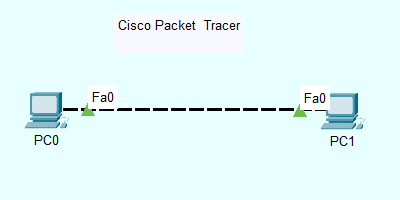
\includegraphics[width=\textwidth]{P2PPacketTracer.png}
        \caption{Point-to-Point in Packet Tracer}
        \label{fig:pt_scenario1}
    \end{subfigure}
    \hfill
    \begin{subfigure}[b]{0.48\textwidth}
        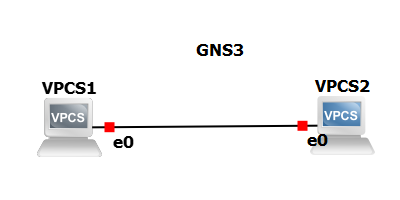
\includegraphics[width=\textwidth]{P2PGNS3.png}
        \caption{Point-to-Point in GNS3}
        \label{fig:gns3_scenario1}
    \end{subfigure}
    \caption[Scenario 1 in beide tools.]{\label{fig:scenario1}Scenario~1 uitgevoerd in zowel Packet Tracer als GNS3.}
\end{figure}



Twee eindapparaten werden rechtstreeks met elkaar verbonden via één UTP-kabel. In \textbf{Packet Tracer} maakten we hiervoor gebruik van twee standaard-pc’s met de namen \texttt{PC0} en \texttt{PC1}. In \textbf{GNS3} stelden we een gelijkaardige situatie voor, maar in plaats van gewone pc’s gebruikten we de \textbf{Virtual PC Simulator (VPCS)}, een lichtgewicht virtuele host die enkel basisnetwerkfunctionaliteit ondersteunt (zoals IP-configuratie, \texttt{ping} en \texttt{traceroute}). VPCS is handig omdat het vrijwel geen resources verbruikt, terwijl het toch toelaat om IP-verkeer te genereren. We noemden ze \texttt{VPCS1} en \texttt{VPCS2}.


\subsection{\IfLanguageName{dutch}{Configuratie in Packet Tracer}{Configuration in Packet Tracer}}
Twee \textbf{pc-iconen} werden op het canvas geplaatst en met elkaar verbonden via een \textbf{Copper Cross-over kabel}. Deze kabel wordt door Packet Tracer doorgaans automatisch geselecteerd bij een verbinding tussen twee pc’s.

Op \texttt{PC0} werd via \texttt{Desktop > IP Configuration} de volgende configuratie ingevoerd:
\begin{itemize}
    \item IP-adres: \texttt{10.0.0.1}
    \item Subnetmasker: \texttt{255.255.255.0}
    \item Gateway: leeg gelaten (niet vereist)
\end{itemize}

Op \texttt{PC1} werd de configuratie als volgt ingesteld:
\begin{itemize}
    \item IP-adres: \texttt{10.0.0.2}
    \item Subnetmasker: \texttt{255.255.255.0}
\end{itemize}

Deze instellingen bleken voldoende. Vervolgens werd op \texttt{PC0}, via het \texttt{Command Prompt} (te vinden onder het tabblad Desktop), het commando \texttt{ping 10.0.0.2} uitgevoerd.

De ping-resultaten waren onmiddellijk positief: de echo-replies keerden terug met \texttt{tijd = 0 ms, TTL = 128}. Hiermee werd de \textbf{connectiviteit succesvol aangetoond}. Verdere configuratie was niet vereist binnen Packet Tracer.

\textit{(Opmerking: Packet Tracer simuleert op de achtergrond automatisch de link-negotiatie en mediadetectie. Dit proces verloopt vrijwel onmiddellijk.)}

\subsection{\IfLanguageName{dutch}{Configuratie in GNS3}{Configuration in GNS3}}

In GNS3 werd gebruikgemaakt van de \textbf{VPCS-functionaliteit} (Virtual PC Simulator). Standaard zijn zes instanties beschikbaar, die via \textit{drag-and-drop} op het canvas geplaatst kunnen worden. Voor dit scenario werden er twee gebruikt.

Een verbinding werd tot stand gebracht tussen \texttt{VPCS1} en \texttt{VPCS2}. In GNS3 wordt dit weergegeven als een eenvoudige lijn, zonder dat een mediumtype hoeft te worden gekozen; de verbinding wordt impliciet als \textbf{ethernetlink} geïnterpreteerd.

Na het starten van de VPCS-nodes (een proces dat slechts een fractie van een seconde in beslag neemt), verschenen voor beide hosts consolevensters. In het console van \texttt{VPCS1} werd het volgende ingevoerd:

\begin{verbatim}
    ip 10.0.0.1/24
\end{verbatim}

Hiermee werd het IP-adres inclusief subnetmasker ingesteld. Omdat beide apparaten zich in hetzelfde subnet bevinden, was geen gateway nodig. In het consolevenster van \texttt{VPCS2} werd ingevoerd:

\begin{verbatim}
    ip 10.0.0.2/24
\end{verbatim}

Vervolgens werd op \texttt{VPCS1} de connectiviteit getest met het commando:

\begin{verbatim}
    ping 10.0.0.2
\end{verbatim}

Vervolgens werd op \texttt{VPCS1} de connectiviteit getest met het commando:

\begin{verbatim}
    ping 10.0.0.2
\end{verbatim}

Alle pingverzoeken kregen een antwoord. De gemeten tijden waren 0.49 ms, 0.92 ms, 0.80 ms, 0.33 ms en 1.63 ms. De eerste reactie kwam onmiddellijk, wat erop wijst dat de ARP-resolutie snel werd uitgevoerd. Er ging geen enkel pakket verloren, en de antwoordtijden waren laag en regelmatig. Dit wijst op een goed werkende point-to-pointverbinding.

De TTL-waarde van 64 geeft aan dat beide hosts zich in hetzelfde subnet bevinden.


\subsection{\IfLanguageName{dutch}{Opmerkingen verschil:}{Opmerkingen verschil:}}
\begin{figure}[H]
    \centering
    \begin{subfigure}[b]{0.48\textwidth}
        \centering
        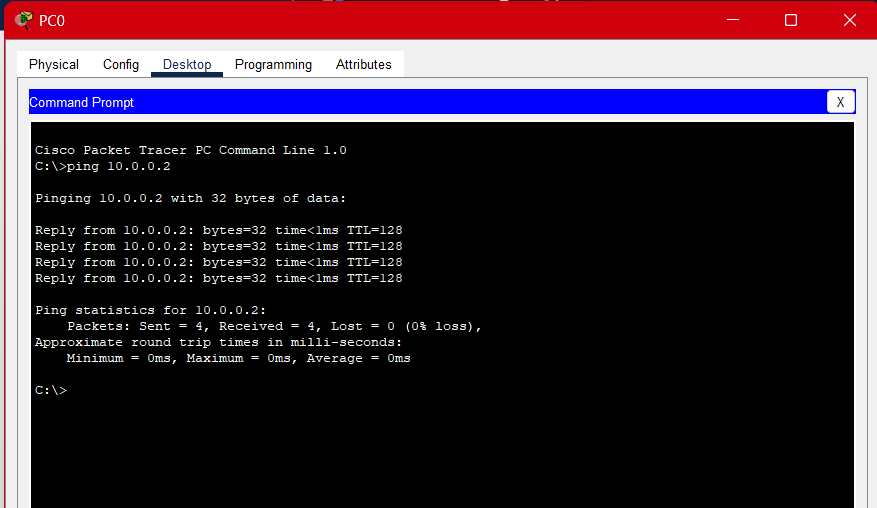
\includegraphics[width=\textwidth]{P2pPacketTracerPing.png}
        \caption{Ping-resultaat in Packet Tracer}
        \label{fig:ping_pt}
    \end{subfigure}
    \hfill
    \begin{subfigure}[b]{0.48\textwidth}
        \centering
        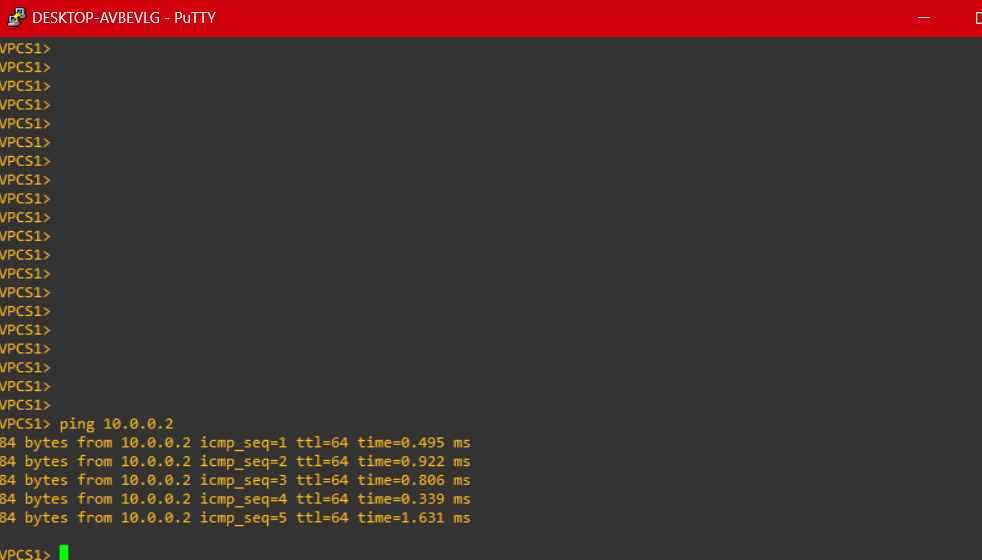
\includegraphics[width=\textwidth]{P2pGNS3Ping.png}
        \caption{Ping-resultaat in GNS3}
        \label{fig:ping_gns3}
    \end{subfigure}
    \caption[Vergelijking van ping resultaten tussen Packet Tracer en GNS3]{Resultaten van het uitvoeren van een \texttt{ping} tussen twee pc’s in een point-to-point scenario in zowel Packet Tracer als GNS3.}
    \label{fig:ping_pt_gns3}
\end{figure}

Scenario 1 functioneerde correct in zowel \textbf{Packet Tracer} als \textbf{GNS3}. In beide simulatieomgevingen kon een eenvoudige point-to-pointverbinding tussen twee hosts succesvol worden opgezet en getest.

\vspace{0.3cm}

Beide tools leverden uiteindelijk succesvolle netwerkconnectiviteit op, maar tijdens het gebruik kwamen er enkele kleine verschillen naar voren. Packet Tracer maakt vooral gebruik van een grafische interface, waarbij IP-instellingen via vensters en dropdownmenu’s worden ingevoerd. GNS3 daarentegen gebruikt bij VPCS een command line-interface (CLI). Voor absolute beginners kan de grafische benadering in Packet Tracer toegankelijker zijn, terwijl GNS3 meer inzicht biedt in onderliggende netwerkprocessen.

\vspace{0.3cm}

Een opvallend verschil is hoe de pingresultaten worden weergegeven. In Packet Tracer werden alle antwoorden onmiddellijk gegeven, telkens met een gemelde tijd van 0 ms. In GNS3 varieerden de tijden tussen 0.3 en 1.6 ms, wat realistischer is en beter aansluit bij het gedrag van een echt netwerk. Hoewel in dit geval de eerste ping meteen succesvol was, komt de ARP-resolutie normaal gesproken expliciet naar voren. In Packet Tracer blijft dat proces verborgen, tenzij de Simulation Mode wordt ingeschakeld.


\vspace{0.3cm}

De uitvoeringstijd en systeembelasting waren bij beide tools ongeveer gelijk. In zowel Packet Tracer als GNS3 verliep de configuratie vlot, zonder merkbaar tijdsverschil. GNS3’s VPCS gebruikte nauwelijks systeembronnen en had geen meetbare impact op de CPU.

\vspace{0.3cm}

Ook de TTL-waarden verschilden: Packet Tracer gebruikte standaard 128, zoals bij Windows-pc’s. GNS3 past dit aan op het type host; VPCS gedraagt zich als een Linux-systeem en gebruikt daardoor een TTL van 64. Dit maakt de simulatie realistischer. 

\vspace{0.3cm}

Beide tools voldeden aan de vereisten voor dit basisnetwerkscenario. 


\section{\IfLanguageName{dutch}{Scenario 2 – Lokaal netwerk met switch en router}{Scenario 2 – Local Network with Switch and Router}}

\label{sec:scenario2}



\subsection{\IfLanguageName{dutch}{Topologie}{Topology}}
\label{sec:topologie-scenario2}

\begin{figure}[H]
    \centering
    \begin{subfigure}[b]{0.48\textwidth}
        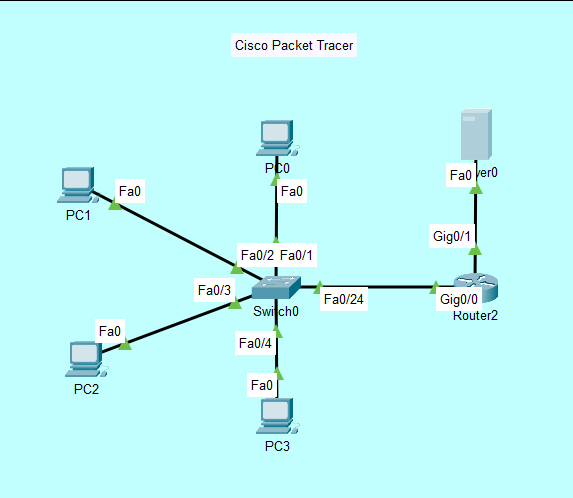
\includegraphics[width=\textwidth]{Sen2PacketTracerTopologie.png}
        \caption{Scenario 2 in Packet Tracer}
        \label{fig:pt_scenario2}
    \end{subfigure}
    \hfill
    \begin{subfigure}[b]{0.48\textwidth}
        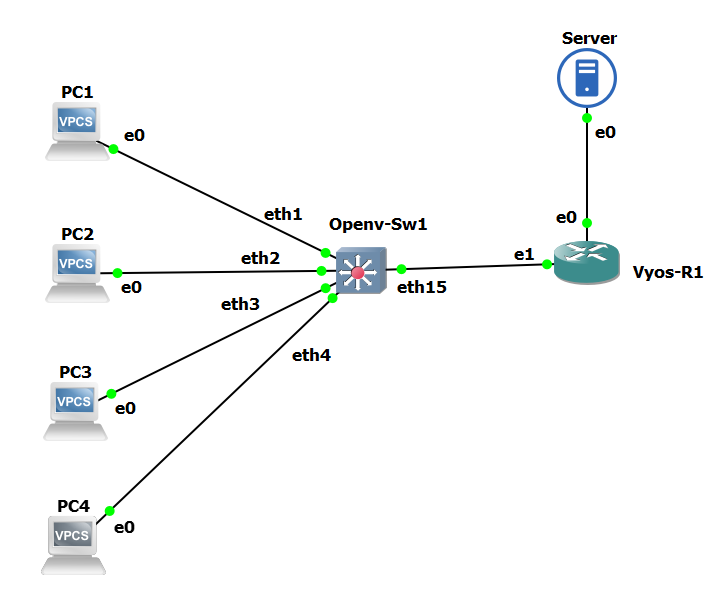
\includegraphics[width=\textwidth]{Sen2GNS3Topologie.png}
        \caption{Scenario 2 in GNS3}
        \label{fig:gns3_scenario2}
    \end{subfigure}
    \caption[Scenario 2 in beide tools.]{\label{fig:scenario2}Scenario~2 uitgevoerd in zowel Packet Tracer als GNS3 met dezelfde netwerkstructuur.}
\end{figure}


In dit scenario stellen we een eenvoudige \textbf{bedrijfsnetwerkomgeving} voor, waarbij meerdere pc’s via een switch zijn verbonden met een router die als gateway fungeert naar een extern netwerk.

\vspace{0.3cm}

Zie Figuur~\ref{fig:scenario2} voor een schematische weergave van de opstelling. In zowel \textbf{Packet Tracer} als \textbf{GNS3} werd dezelfde netwerktopologie opgebouwd: vier pc’s zijn verbonden met één switch, die via een trunkverbinding (nodig voor het doorsturen van verkeer van meerdere VLAN’s) gekoppeld is aan een router. Op de router zijn subinterfaces geconfigureerd voor twee VLAN’s: \texttt{VLAN10} voor de eerste twee pc’s en \texttt{VLAN20} voor de derde en vierde pc. De router fungeert als gateway voor beide VLAN’s volgens het Router-on-a-Stick-principe.



\vspace{0.3cm}

De buiteninterface van de router is verbonden met een gesimuleerd extern netwerk dat het internet voorstelt, met daarin een server met IP-adres \texttt{8.8.8.8}. De router voert NAT-overload uit om interne clients toegang te geven tot het externe netwerk, en fungeert ook als DHCP-server voor beide VLAN’s. Daarnaast is er een ACL (in Packet Tracer) en een firewall (in GNS3) ingesteld waarbij alleen toestellen in VLAN20 ICMP-verkeer (zoals pings) mogen sturen naar de externe server. Verkeer vanuit VLAN10 wordt daarbij geblokkeerd. Deze opstelling biedt de mogelijkheid om het gedrag van netwerktoegang en verkeersfiltering in verschillende situaties  te observeren en te vergelijken. 


In \textbf{GNS3} werd dezelfde topologie opgebouwd als in Packet Tracer, maar met open-source componenten zoals \texttt{VyOS} en \texttt{Open vSwitch}, aangezien officiële Cisco IOS-images enkel via een licentie verkregen kunnen worden.


\textbf{Extra componenten:}
\begin{itemize}
    \item De router fungeert als DHCP-server en wijst automatisch IP-adressen toe aan de pc’s in beide VLAN’s.
    \item NAT-overload is geconfigureerd zodat interne pc’s toegang krijgen tot het externe netwerk via één publiek IP-adres.
    \item Een ACL in \textbf{Packet Tracer} en een firewall in \textbf{GNS3} bepaalt dat enkel bepaalde hosts (zoals in VLAN20) ICMP-verkeer naar een specifieke externe server mogen sturen, terwijl ander ICMP-verkeer wordt geblokkeerd.
\end{itemize}

\vspace{0.5cm}

\subsubsection{\IfLanguageName{dutch}{Configuratie in Packet Tracer}{Configuration in Packet Tracer}}

In \textbf{Packet Tracer} werden vier pc’s toegevoegd, samen met één switch (type \texttt{2960}) en een \texttt{2911}-router. PC0 en PC1 zijn verbonden met VLAN10, PC2 en PC3 met VLAN20. Daarnaast werd een server toegevoegd aan de buiteninterface van de router om het externe netwerk te simuleren. Deze server kreeg het IP-adres \texttt{8.8.8.8}.

\textbf{1. Switchconfiguratie (Cisco 2960):}
\begin{verbatim}
    enable
    configure terminal
    
    vlan 10
    name Client10
    exit
    
    vlan 20
    name Client20
    exit
    
    vlan 100
    name Trunk
    exit
    
    interface range fa0/1 - 2
    switchport mode access
    switchport access vlan 10
    exit
    
    interface range fa0/3 - 4
    switchport mode access
    switchport access vlan 20
    exit
    
    interface fa0/24
    switchport mode trunk
    switchport trunk native vlan 100
    end
    
    
\end{verbatim}

\textbf{2. Routerconfiguratie (Cisco 2811):}

\begin{verbatim}
    interface g0/0.10
    encapsulation dot1Q 10
    ip address 192.168.10.254 255.255.255.0
    ip nat inside
    ip access-group 101 in
    exit
    
    interface g0/0.20
    encapsulation dot1Q 20
    ip address 192.168.20.254 255.255.255.0
    ip nat inside
    ip access-group 101 in
    exit
\end{verbatim}

\textbf{Stap 2: Hoofdinterface activeren}

\begin{verbatim}
    interface g0/0
    no shutdown
    exit
\end{verbatim}

\textbf{Stap 3: WAN-interface (naar internet) configureren}

\begin{verbatim}
    interface g0/1
    ip address 8.8.8.1 255.255.255.0
    ip nat outside
    ip access-group 101 in
    no shutdown
    exit
\end{verbatim}

\textbf{Stap 4: DHCP-configuratie}

De router krijgt twee DHCP pools mee, één per VLAN. Elke pool deelt IP-adressen uit binnen het subnet van het respectieve VLAN.

\begin{verbatim}
    ip dhcp pool NET10
    network 192.168.10.0 255.255.255.0
    default-router 192.168.10.254
    dns-server 8.8.8.8
    exit
    
    ip dhcp pool NET20
    network 192.168.20.0 255.255.255.0
    default-router 192.168.20.254
    dns-server 8.8.8.8
    exit
\end{verbatim}

\textbf{Stap 5: NAT-configuratie}

Hier wordt NAT overload ingesteld zodat alle interne hosts via \texttt{G0/1} toegang tot internet kunnen krijgen.

\begin{verbatim}
    access-list 1 permit 192.168.0.0 0.0.255.255
    ip nat inside source list 1 interface g0/1 overload
\end{verbatim}

\textbf{Stap 6: Access Control List (ACL)}

ACL 101 zorgt ervoor dat alleen VLAN 20 (192.168.20.0/24) toegang heeft tot de server \texttt{8.8.8.8}. VLAN 10 wordt geblokkeerd. Alle ander verkeer wordt toegestaan.

\begin{verbatim}
    access-list 101 permit ip 192.168.20.0 0.0.0.255 host 8.8.8.8
    access-list 101 deny ip 192.168.10.0 0.0.0.255 host 8.8.8.8
    access-list 101 permit ip any any
\end{verbatim}


\subsubsection{\IfLanguageName{dutch}{Configuratie in GNS3}{Configuration in GNS3}}

In \textbf{GNS3} werd dezelfde topologie opgebouwd als in Packet Tracer. Vier \texttt{VPCS}-hosts zijn via \texttt{Open vSwitch} verbonden met een \texttt{VyOS}-router. PC1 en PC2 behoren tot \texttt{VLAN10}, PC3 en PC4 tot \texttt{VLAN20}. De trunkverbinding loopt van poort \texttt{eth15} op de switch naar \texttt{eth1} op de router. De WAN-verbinding verloopt via \texttt{eth0} naar een externe server (\texttt{8.8.8.8}). 

De structuur en werking zijn identiek aan de Packet Tracer-topologie, maar worden hier gerealiseerd met open-source tools.


\textbf{1. Switchconfiguratie (Open vSwitch):}
\begin{verbatim}
    # VLAN 10 - Access
    ovs-vsctl set port eth1 tag=10
    ovs-vsctl set port eth2 tag=10
    
    # VLAN 20 - Access
    ovs-vsctl set port eth3 tag=20
    ovs-vsctl set port eth4 tag=20
    
    # Trunk naar VyOS-router
    ovs-vsctl set port eth15 trunks=10,20
\end{verbatim}

\textbf{2. Routerconfiguratie (VyOS):}
\begin{verbatim}
    configure
    
    # WAN-interface (naar internet)
    set interfaces ethernet eth0 address '8.8.8.1/24'
    
    # Subinterfaces voor VLAN 10 en 20 op eth1
    set interfaces ethernet eth1 vif 10 address '192.168.10.254/24'
    set interfaces ethernet eth1 vif 20 address '192.168.20.254/24'
\end{verbatim}

\textbf{Stap 2: NAT-configuratie}
\begin{verbatim}
    set nat source rule 100 description 'NAT voor LAN naar WAN'
    set nat source rule 100 source address '192.168.0.0/16'
    set nat source rule 100 outbound-interface name eth0
    set nat source rule 100 translation address masquerade
\end{verbatim}

\textbf{Stap 3: DHCP-configuratie}
\begin{verbatim}
    # VLAN 10
    set service dhcp-server shared-network-name VLAN10 subnet 192.168.10.0/24 subnet-id 1
    set service dhcp-server shared-network-name VLAN10 subnet 192.168.10.0/24 range 0 start '192.168.10.10'
    set service dhcp-server shared-network-name VLAN10 subnet 192.168.10.0/24 range 0 stop '192.168.10.100'
    set service dhcp-server shared-network-name VLAN10 subnet 192.168.10.0/24 range 0 option default-router '192.168.10.254'
    set service dhcp-server shared-network-name VLAN10 subnet 192.168.10.0/24 range 0 option name-server '8.8.8.8'
    
    # VLAN 20
    set service dhcp-server shared-network-name VLAN20 subnet 192.168.20.0/24 subnet-id 2
    set service dhcp-server shared-network-name VLAN20 subnet 192.168.20.0/24 range 0 start '192.168.20.10'
    set service dhcp-server shared-network-name VLAN20 subnet 192.168.20.0/24 range 0 stop '192.168.20.100'
    set service dhcp-server shared-network-name VLAN20 subnet 192.168.20.0/24 range 0 option default-router '192.168.20.254'
    set service dhcp-server shared-network-name VLAN20 subnet 192.168.20.0/24 range 0 option name-server '8.8.8.8'
\end{verbatim}

\textbf{Stap 4: Firewallconfiguratie (ter vervanging van ACL)}
\begin{verbatim}
    set firewall ipv4 name VLAN-ACCESS rule 10 action 'accept'
    set firewall ipv4 name VLAN-ACCESS rule 10 source address '192.168.20.0/24'
    set firewall ipv4 name VLAN-ACCESS rule 10 destination address '8.8.8.8'
    
    set firewall ipv4 name VLAN-ACCESS rule 20 action 'drop'
    set firewall ipv4 name VLAN-ACCESS rule 20 source address '192.168.10.0/24'
    set firewall ipv4 name VLAN-ACCESS rule 20 destination address '8.8.8.8'
    
    set firewall ipv4 name VLAN-ACCESS rule 30 action 'accept'
\end{verbatim}

\textbf{Stap 5: Zones definiëren}
\begin{verbatim}
    set firewall zone LAN default-action drop
    set firewall zone LAN member interface eth1.10
    set firewall zone LAN member interface eth1.20
    
    set firewall zone WAN default-action drop
    set firewall zone WAN member interface eth0
    
    set firewall zone WAN from LAN firewall name VLAN-ACCESS
    set firewall zone WAN from LAN default-action drop
    
    commit
    save
\end{verbatim}


\subsection{\IfLanguageName{dutch}{Opmerkingen verschil:}{Opmerkingen verschil:}}

In scenario 2 werden de verschillen tussen beide tools al snel duidelijk. In GNS3 kan men niet onmiddellijk beginnen met het opbouwen van een topologie. Eerst moeten geschikte VyOS- en Open vSwitch-images worden gedownload en gekoppeld aan de GNS3-VM. Pas daarna kunnen de netwerkcomponenten worden toegevoegd en geconfigureerd. Hoewel dit met een duidelijke handleiding goed uitvoerbaar is, vraagt het meer technische voorbereiding, inzicht en extra tijd dan bij Cisco Packet Tracer. In Packet Tracer zijn de Cisco-router en -switch direct beschikbaar, waardoor het integreren van pc’s, switches en routers snel en zonder bijkomende configuratie verloopt.

\vspace{0.3cm}

Ook op het vlak van systeemprestaties zijn er verschillen merkbaar. Het opstarten van virtuele apparaten in GNS3 vraagt meer rekenkracht. De VyOS-router en Open vSwitch veroorzaken een tijdelijke piek in het CPU-gebruik, die na het volledig opstarten weer terugvalt naar een stabiel niveau. Packet Tracer werkt met interne simulatie waarbij apparaten onmiddellijk beschikbaar zijn en de belasting van het systeem minimaal blijft. Dit maakt Packet Tracer bijzonder efficiënt voor eenvoudige netwerkscenario’s. GNS3 biedt daarentegen realistischer netwerkgedrag. Alles start iets trager op, maar ik had wel meer controle en kon makkelijker zien waar iets fout liep.

\vspace{0.3cm}

Wat betreft de tijdsbesteding viel op dat het configuratieproces in GNS3 duidelijk meer tijd vroeg dan in Cisco Packet Tracer. Voor scenario 2 kon het volledige netwerk in Packet Tracer binnen 15 minuten worden opgebouwd en getest. In GNS3 liep de benodigde tijd op tot 30 tot 35 minuten. Deze extra tijd was vooral het gevolg van het opstarten van de virtuele componenten: zowel de VyOS-router als Open vSwitch moesten volledig actief zijn voordat de configuratie kon beginnen. Voor de rest waren de configuratiestappen en het eindresultaat identiek in beide omgevingen. Dezelfde configuratie kon zonder aanpassingen worden toegepast in zowel Packet Tracer als GNS3, met vergelijkbare werking.

\vspace{0.3cm}

\begin{figure}[H]
    \centering
    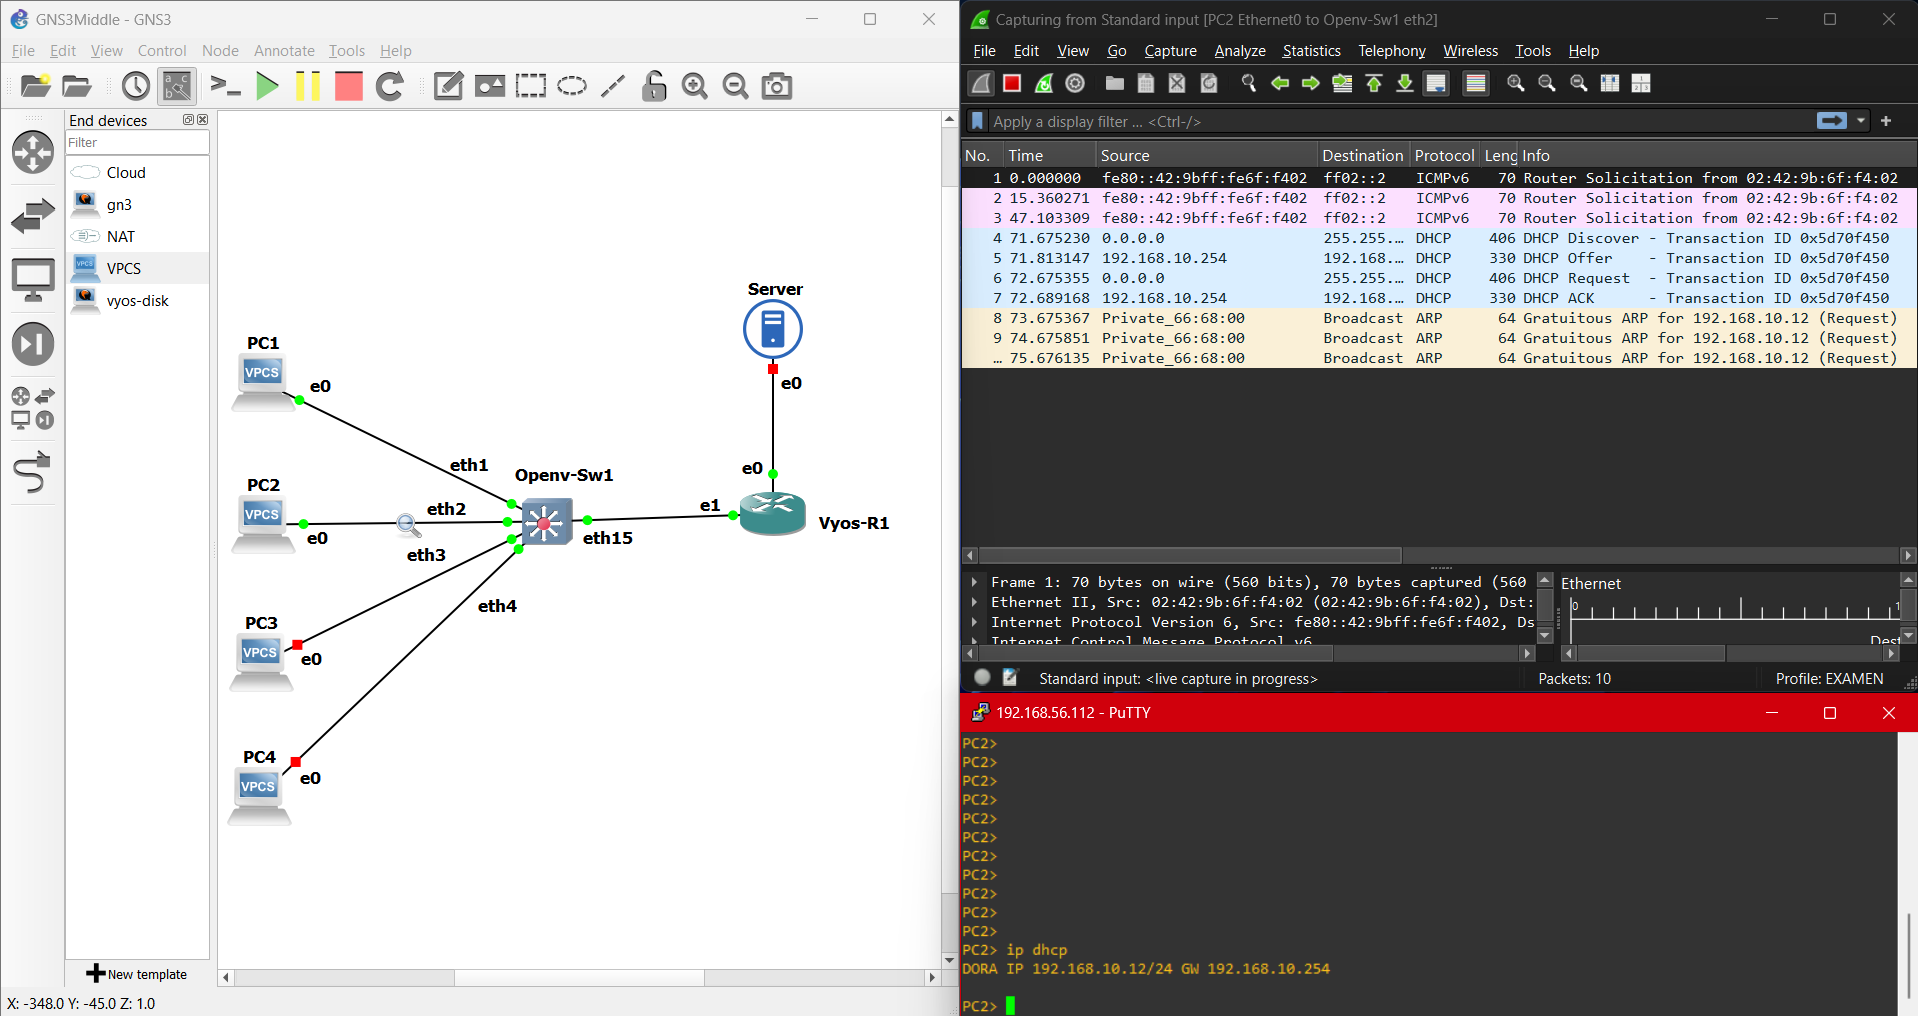
\includegraphics[width=0.7\textwidth]{WeergaveDHCPGns3.png}
    \caption{DHCP proces zichtbaar in GNS3 via packet capture.}
    \label{fig:dhcp_gns3}
\end{figure}


Een bijkomend voordeel van werken in GNS3 is dat het mogelijk maakt om netwerkverkeer tot in detail te observeren. Zoals weergegeven in afbeelding ~\ref{fig:dhcp_gns3} , verschijnen na het opstarten van de router automatisch verschillende netwerkberichten in de packet capture. PC2 stuurt eerst een verzoek uit om een router in het netwerk te vinden. Kort daarna start het volledige DHCP proces. De computer vraagt een IP-adres aan en ontvangt vervolgens een geldig adres samen met de standaardgateway. Dit bevestigt dat de DHCP-configuratie correct is uitgevoerd.

\vspace{0.3cm}

\begin{figure}[H]
    \centering
    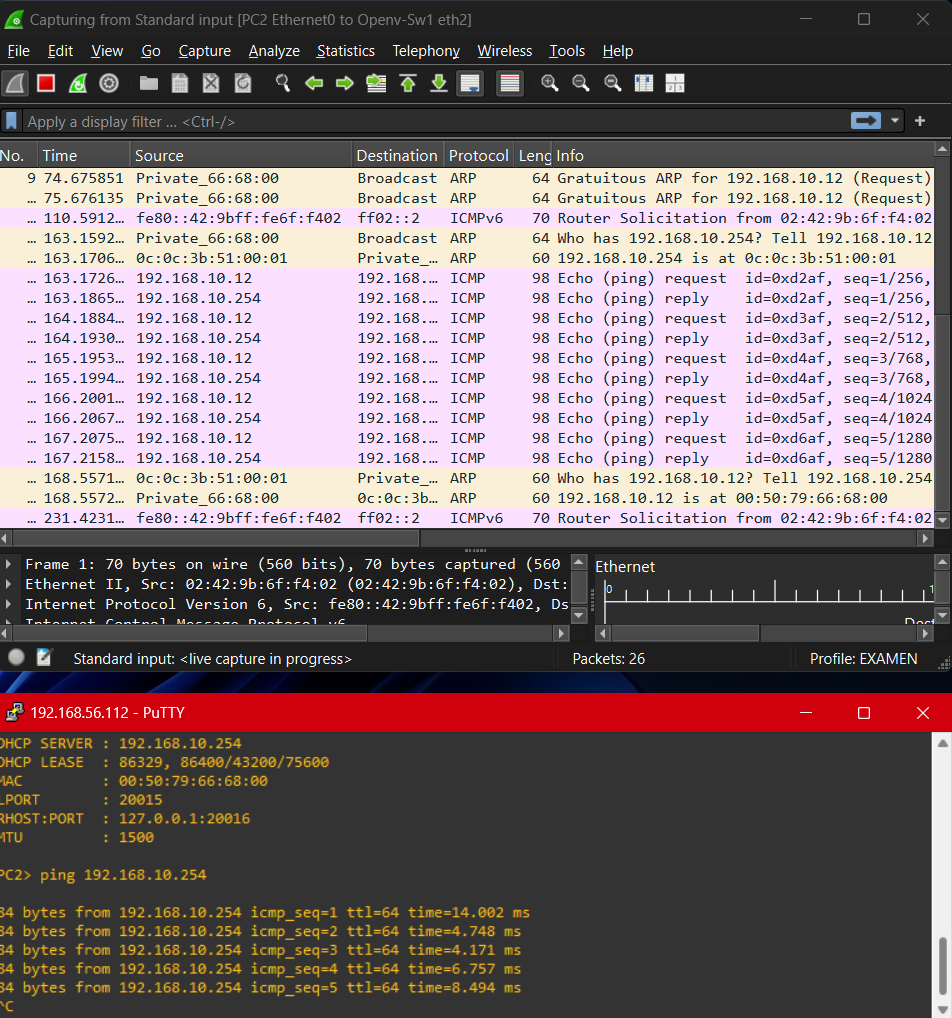
\includegraphics[width=0.7\textwidth]{PingverkeerTussenPCEnRouter.png}
    \caption{Pingverkeer tussen PC2 en de router in GNS3.}
    \label{fig:ping_gns3}
\end{figure}

In afbeelding ~\ref{fig:ping_gns3} wordt dit verder getest met een ping naar het adres van de router. Daarbij zijn zowel het pingbericht als het antwoord zichtbaar, samen met de tijd die nodig is om te reageren. Deze manier van testen benadert sterk de werking van een echt netwerk.

\vspace{0.3cm}

In Cisco Packet Tracer verloopt dit proces op basis van vooraf gesimuleerde processen. De configuratie werkt functioneel, maar de communicatie tussen apparaten wordt niet zichtbaar gemaakt. De DHCP-aanvraag gebeurt automatisch op de achtergrond, zonder dat de tussenliggende stappen of datapakketten weergegeven worden. Ook bij een ping zie je enkel het eindresultaat, zonder details over het verloop. Hierdoor is het moeilijker om fouten op te sporen of inzicht te krijgen in hoe het netwerk reageert. GNS3 biedt in dat opzicht meer transparantie en realisme, en is daardoor beter geschikt om netwerkprocessen grondig te analyseren.






\section{\IfLanguageName{dutch}{Scenario 3 – Complex netwerk (CCNA-Niveau 3)}{Scenario 3 – Complex netwerk (CCNA-Niveau 3}}
\label{sec:scenario3}

\subsection{\IfLanguageName{dutch}{Topologie Scenario 3}{Topology Scenario 3}}
\label{sec:topologie-scenario3}

\begin{figure}[H]
    \centering
    \begin{subfigure}[b]{0.48\textwidth}
        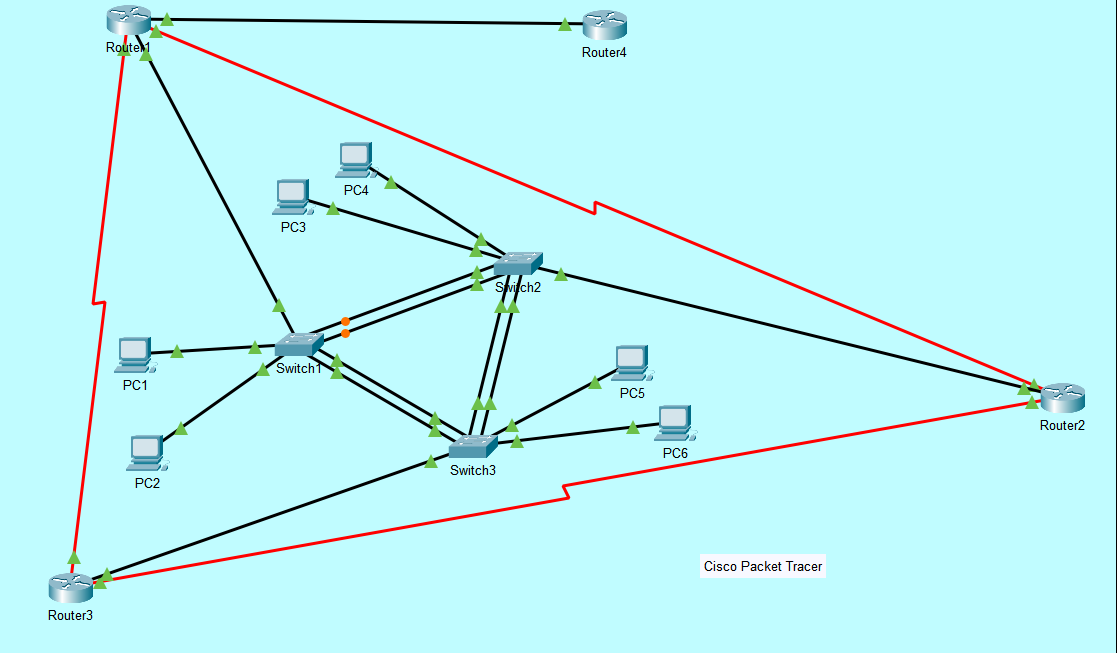
\includegraphics[width=\textwidth]{Sen3PacketTracerTopologie.png}
        \caption{Scenario 3 in Packet Tracer}
        \label{fig:pt_scenario3}
    \end{subfigure}
    \hfill
    \begin{subfigure}[b]{0.48\textwidth}
        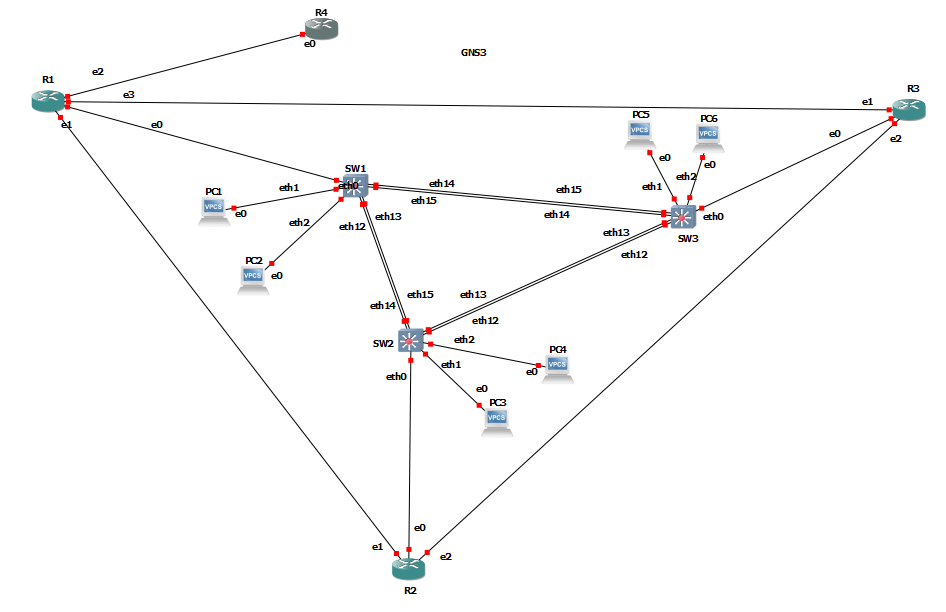
\includegraphics[width=\textwidth]{Sen3Gns3Topologie.png}
        \caption{Scenario 3 in GNS3}
        \label{fig:gns3_scenario3}
    \end{subfigure}
    \caption[Scenario 3 in beide tools.]{\label{fig:scenario3}Scenario~3 uitgevoerd in zowel Packet Tracer als GNS3 met vergelijkbare netwerkstructuur.}
\end{figure}



In dit scenario bouwen we een uitgebreid netwerk dat drie afzonderlijke locaties met elkaar verbindt. De structuur van deze opstelling wordt weergegeven in Figuur~\ref{fig:scenario3}.

\vspace{0.3cm}

Elke locatie beschikt over een eigen router (R1, R2 en R3) en een eigen switch (SW1, SW2 en SW3). De routers zijn verbonden volgens een driehoekstopologie, waardoor er steeds meerdere paden beschikbaar zijn tussen de verschillende sites. Deze topologie is opgezet om de werking van OSPF-routing binnen een redundante netwerkstructuur te demonstreren.

\vspace{0.3cm}

Elke switch is geconfigureerd met twee VLAN’s: VLAN10 en VLAN20. In elk VLAN bevindt zich één pc, zodat elke locatie logisch is opgesplitst in aparte afdelingen of gebruikersgroepen.

\vspace{0.3cm}

Router R1 is verbonden met een vierde router (R4) die als internetgateway fungeert. Om internettoegang mogelijk te maken, vertaalt R1 de interne IP-adressen naar een publiek IP-adres via NAT-overload.

\vspace{0.3cm}

Op alle drie de routers is OSPF ingesteld voor dynamische routering. De IP-adrestoewijzing gebeurt via twee DHCP servers: R2 beheert VLAN10 en R3 verzorgt VLAN20.


\vspace{0.3cm}

Elke switch is gekoppeld aan zijn router en ook rechtstreeks verbonden met de andere switches via trunklinks en EtherChannels. Door deze opstelling ontstaat een driehoek op laag 2. STP, dat standaard actief is, voorkomt automatisch netwerkloops door één van de verbindingen te blokkeren.


\subsubsection{\IfLanguageName{dutch}{Configuratie in Packet Tracer}{Configuration in Packet Tracer}}
\label{sec:configuratie-PacketTracer}

De volgende configuratie werd toegepast op de routers en switches in Scenario~2. Aangezien veel instellingen gelijkaardig zijn, zijn de configuratieblokken gegroepeerd per toesteltype.

\vspace{0.3cm}

\paragraph{Router R1: Gateway + NAT + DHCP + OSPF}
\begin{verbatim}
    interface g0/0.10
    encapsulation dot1Q 10
    ip address 10.1.10.254 255.255.255.0
    ip nat inside
    ip access-group 101 in
    exit
    
    interface g0/0.20
    encapsulation dot1Q 20
    ip address 10.1.20.254 255.255.255.0
    ip nat inside
    ip access-group 101 in
    exit
    
    interface g0/0
    no shutdown
    exit
    
    interface g0/1
    ip address 192.0.2.1 255.255.255.0
    ip nat outside
    no shutdown
    exit
    
    interface s0/3/0
    ip address 10.10.12.1 255.255.255.252
    clock rate 64000
    ip nat inside
    no shutdown
    exit
    
    interface s0/3/1
    ip address 10.10.13.1 255.255.255.252
    ip nat inside
    no shutdown
    exit
    
    ip dhcp excluded-address 10.1.10.1 10.1.10.99
    ip dhcp excluded-address 10.1.20.1 10.1.20.99
    
    access-list 1 permit 10.0.0.0 0.255.255.255
    ip nat inside source list 1 interface g0/1 overload
    
    ip route 0.0.0.0 0.0.0.0 192.0.2.254
    
    router ospf 1
    network 10.0.0.0 0.255.255.255 area 0
    network 10.10.12.0 0.0.0.3 area 0
    network 10.10.13.0 0.0.0.3 area 0
    network 192.0.2.0 0.0.0.255 area 0
    default-information originate
\end{verbatim}

\vspace{0.3cm}
\paragraph{Routers R2 en R3 (gelijkend, met aangepaste IP's)}
(Sterk gelijkaardig aan R1, maar met eigen subnetten)
\textit{Voorbeeld R2:}
\begin{verbatim}
    interface g0/0.10
    encapsulation dot1Q 10
    ip address 10.2.10.254 255.255.255.0
    ip nat inside
    exit
    
    interface s0/3/0
    ip address 10.10.12.2 255.255.255.252
    ip nat inside
    no shutdown
    exit
    
    ip dhcp pool VLAN10
    network 10.2.10.0 255.255.255.0
    default-router 10.2.10.254
    dns-server 8.8.8.8
    
    router ospf 1
    network 10.10.12.0 0.0.0.3 area 0
\end{verbatim}

\vspace{0.3cm}

\paragraph{Router R4: Internet-router}
\begin{verbatim}
    interface g0/0
    ip address 192.0.2.254 255.255.255.0
    no shutdown
    exit
    ip route 0.0.0.0 0.0.0.0 GigabitEthernet0/0
    
    ip route 0.0.0.0 0.0.0.0 g0/0
\end{verbatim}

\vspace{0.3cm}
\paragraph{Switch SW1–SW3: VLAN-configuratie + Trunk + EtherChannel}
(SW1 voorbeeld)
\begin{verbatim}
    vlan 10
    name Client10
    vlan 20
    name Client20
    
    interface fa0/2
    switchport mode access
    switchport access vlan 10
    exit
    interface fa0/3
    switchport mode access
    switchport access vlan 20
    exit
    
    interface fa0/1
    switchport mode trunk
    switchport trunk allowed vlan 10,20
    exit
    
    interface range fa0/23 - 24
    switchport mode trunk
    channel-group 1 mode desirable
    exit
    
    interface Port-channel1
    switchport mode trunk
    switchport trunk allowed vlan 10,20
    exit
\end{verbatim}



\subsubsection{\IfLanguageName{dutch}{Configuratie in GNS3}{Configuration in GNS3}}
\label{sec:configuratie-Gns3}


In GNS3 werd hetzelfde netwerk nagebouwd met \textbf{VyOS-routers} en \textbf{Open vSwitch (OVS)}-switches. De configuratie wordt hieronder per toesteltype weergegeven, waarbij gelijkaardige instellingen gegroepeerd zijn om herhaling te vermijden.

\vspace{0.3cm}
\paragraph{Router R1: Gateway + NAT + DHCP + OSPF}
\begin{verbatim}
    configure
    
    set interfaces ethernet eth0 vif 10 address '10.1.10.254/24'
    set interfaces ethernet eth0 vif 10 description 'VLAN10'
    set interfaces ethernet eth0 vif 20 address '10.1.20.254/24'
    set interfaces ethernet eth0 vif 20 description 'VLAN20'
    set interfaces ethernet eth0 description 'Trunk to Switch'
    set interfaces ethernet eth1 address '192.0.2.1/24'
    set interfaces ethernet eth1 description 'Internet'
    set interfaces ethernet eth2 address '10.10.12.1/30'
    set interfaces ethernet eth3 address '10.10.13.1/30'
    
    set nat source rule 10 source address '10.0.0.0/8'
    set nat source rule 10 outbound-interface 'eth1'
    set nat source rule 10 translation address 'masquerade'
    
    set protocols static route 0.0.0.0/0 next-hop 192.0.2.254
    
    set protocols ospf area 0 network 10.0.0.0/8
    set protocols ospf parameters router-id 1.1.1.1
    set protocols ospf redistribute static
    
    commit
    save
\end{verbatim}

\vspace{0.3cm}
\paragraph{Router R2: DHCP + OSPF}
\begin{verbatim}
    configure
    
    set interfaces ethernet eth0 vif 10 address '10.2.10.254/24'
    set interfaces ethernet eth0 vif 20 address '10.2.20.254/24'
    set interfaces ethernet eth0 description 'Trunk'
    set interfaces ethernet eth1 address '10.10.12.2/30'
    set interfaces ethernet eth2 address '10.10.23.1/30'
    
    set service dhcp-server shared-network-name VLAN10 subnet 10.2.10.0/24 \
    default-router '10.2.10.254' dns-server '8.8.8.8' range 0 start '10.2.10.100' stop '10.2.10.200'
    
    set protocols ospf area 0 network 10.0.0.0/8
    set protocols ospf parameters router-id 2.2.2.2
    
    commit
    save
\end{verbatim}

\vspace{0.3cm}
\paragraph{Router R3: DHCP + OSPF}
\begin{verbatim}
    configure
    
    set interfaces ethernet eth0 vif 10 address '10.3.10.254/24'
    set interfaces ethernet eth0 vif 20 address '10.3.20.254/24'
    set interfaces ethernet eth0 description 'Trunk'
    set interfaces ethernet eth1 address '10.10.23.2/30'
    set interfaces ethernet eth2 address '10.10.13.2/30'
    
    set service dhcp-server shared-network-name VLAN20 subnet 10.3.20.0/24 \
    default-router '10.3.20.254' dns-server '8.8.8.8' range 0 start '10.3.20.100' stop '10.3.20.200'
    
    set protocols ospf area 0 network 10.0.0.0/8
    set protocols ospf parameters router-id 3.3.3.3
    
    commit
    save
\end{verbatim}

\vspace{0.3cm}

\paragraph{Router R4: Internet + Statische route}
\begin{verbatim}
    configure
    
    set interfaces ethernet eth0 address '192.0.2.254/24'
    set protocols static route 0.0.0.0/0 next-hop '192.0.2.1'
    
    commit
    save
\end{verbatim}

\vspace{0.3cm}
\paragraph{Switches SW1–SW3: Open vSwitch configuratie (OVS)}
\textit{Voorbeeld voor SW1}
\begin{verbatim}
    # Access ports voor PC1 en PC2
    ovs-vsctl set port eth1 tag=10
    ovs-vsctl set port eth2 tag=20
    
    # Trunk naar Router1
    ovs-vsctl set port eth0 trunks=10,20
    
    # EtherChannel bond1 (naar SW2 via eth12 + eth13)
    ovs-vsctl add-bond br0 bond1 eth12 eth13
    ovs-vsctl set port bond1 trunks=10,20
    
    # EtherChannel bond2 (naar SW3 via eth14 + eth15)
    ovs-vsctl add-bond br0 bond2 eth14 eth15
    ovs-vsctl set port bond2 trunks=10,20
\end{verbatim}

\subsection{\IfLanguageName{dutch}{Opmerkingen verschil:}{Opmerkingen verschil:}}

Scenario 3 was de meest uitgebreide test in deze vergelijking. Het netwerk was opgebouwd uit meerdere routers en switches, waarbij verschillende protocollen werden toegepast. Naast de functionele werking werd ook gekeken naar configuratietijd en systeemprestaties. Daardoor kwamen de verschillen tussen Cisco Packet Tracer en GNS3 duidelijk naar voren.

\vspace{0.3cm}

Tijdens de uitvoering bleek er een significant verschil in de benodigde tijd en systeembelasting tussen beide platforms. In Cisco Packet Tracer kon het volledige netwerk binnen ongeveer 40 minuten worden opgebouwd en getest. De apparaten waren meteen beschikbaar en reageerden vrijwel onmiddellijk, waardoor de configuratie vlot verliep. In GNS3 daarentegen duurde het opzetten van hetzelfde netwerk ongeveer 1 uur en 20 minuten. Deze langere opstarttijd werd, net als in Scenario 2, vooral veroorzaakt door het laden van de virtuele toestellen. De VyOS-router bijvoorbeeld heeft enkele minuten nodig om volledig op te starten, en ook andere componenten moeten eerst actief zijn vooraleer er kon worden gestart met configureren en testen. Dit zorgde voor een merkbare vertraging in de beginfase van het configuratieproces.

\vspace{0.3cm}



Ook op het vlak van systeembelasting kwamen duidelijke verschillen naar voren. Tijdens het opstarten van GNS3 werd het CPU-gebruik gemeten met Taakbeheer op een Windows 11-laptop met een Intel Core i5-1135G7 (quad-core, 8 threads) en 16 GB RAM. De metingen werden driemaal herhaald, telkens met eenzelfde netwerktopologie van tien routers, vier switches en zes pc’s. Daarbij steeg het CPU-gebruik bij het starten van GNS3 tijdelijk tot 100\%. Zodra alle virtuele apparaten actief waren, stabiliseerde het CPU-verbruik tussen 47\% en 69\%, afhankelijk van de netwerkactiviteit. Ter vergelijking: in Packet Tracer bleef het CPU-gebruik in gelijkaardige omstandigheden onder de 20\%. Dit verschil is verklaarbaar, aangezien GNS3 gebruikmaakt van echte virtuele machines en emulatie, terwijl Packet Tracer gesimuleerde apparaten aanstuurt binnen een licht geoptimaliseerde omgeving(zie figuur~\ref{fig:cpu_gns3}).

\vspace{0.3cm}

\begin{figure}[H]
    \centering
    \begin{subfigure}[b]{0.48\textwidth}
        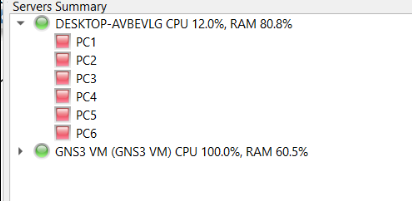
\includegraphics[width=\textwidth]{CpuVerbruik1.png}
        \caption{CPU-gebruik tijdens het opstarten van GNS3}
        \label{fig:cpu_opstart}
    \end{subfigure}
    \hfill
    \begin{subfigure}[b]{0.48\textwidth}
        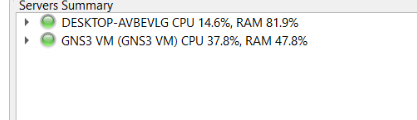
\includegraphics[width=\textwidth]{CpuVerbruik2.png}
        \caption{Gestabiliseerd CPU-gebruik na opstart}
        \label{fig:cpu_na_opstart}
    \end{subfigure}
    \caption[CPU verbruik van GNS3 tijdens Scenario 3.]{\label{fig:cpu_gns3}CPU-verbruik van GNS3 bij het opstarten en na stabilisatie tijdens Scenario~3.}
\end{figure}


Een belangrijk aanvullend voordeel van GNS3, in vergelijking met Packet Tracer, is de mogelijkheid om het volledige OSPF-proces te analyseren via Wireshark. Tijdens een packet capture zijn alle fasen van het protocol zichtbaar, zoals Hello-pakketten, Database Description, Link State Request, Link State Update en Link State Acknowledgement. Dit biedt een gedetailleerd inzicht in het verloop van het routingproces. In Packet Tracer zijn deze stappen niet waarneembaar; daar zijn enkel visuele statusindicatoren beschikbaar, wat de analyse beperkt.(zie figuur~\ref{fig:ospf_wireshark}).

\begin{figure}[H]
    \centering
    
    \begin{subfigure}[b]{\textwidth}
        \centering
        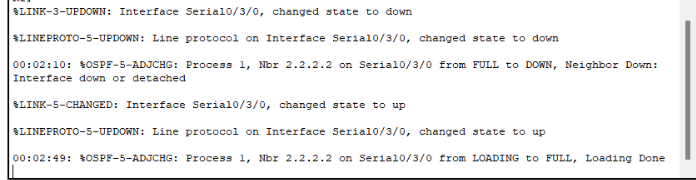
\includegraphics[width=\textwidth]{OSPFBerichten1.png}
        \caption{Packet Tracer: OSPF-berichten op Router 1}
        \label{fig:ospf_r1}
    \end{subfigure}
    
    \vspace{1em}
    
    \begin{subfigure}[b]{\textwidth}
        \centering
        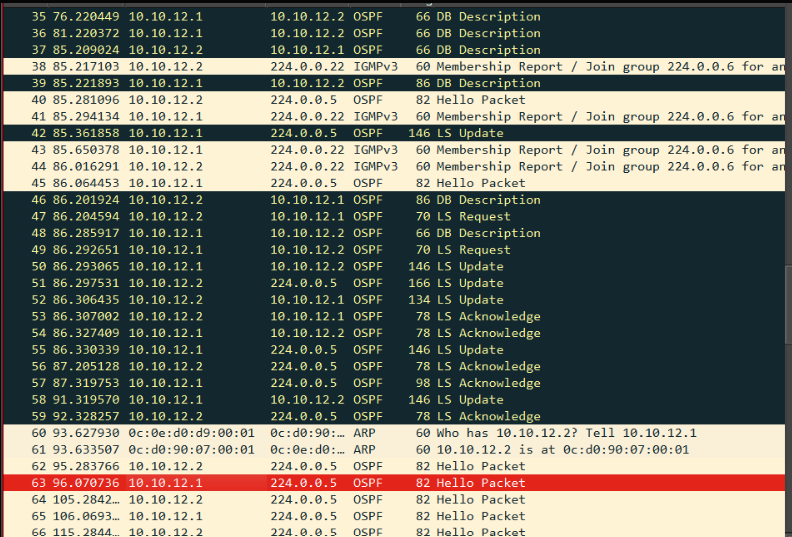
\includegraphics[width=\textwidth]{OSPFBerichten2.png}
        \caption{Wireshark: OSPF-berichten op Router 2}
        \label{fig:ospf_r2}
    \end{subfigure}
    
    \vspace{1em}
    
    \begin{subfigure}[b]{\textwidth}
        \centering
        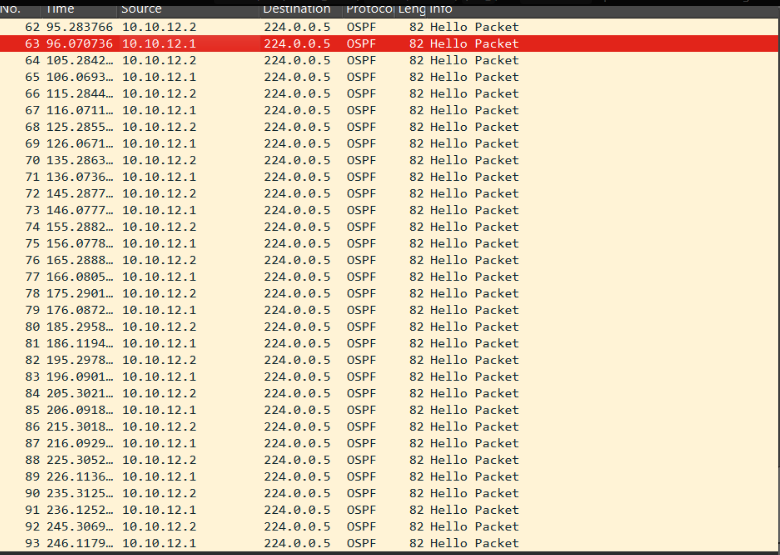
\includegraphics[width=\textwidth]{OSPFBerichten3.png}
        \caption{Wireshark: OSPF-berichten op Router 3}
        \label{fig:ospf_r3}
    \end{subfigure}
    
    \caption[OSPF verkeer zichtbaar via Wireshark in GNS3.]{\label{fig:ospf_wireshark}Weergave van het OSPF-proces via Wireshark in GNS3 op drie verschillende routers. In Packet Tracer zijn deze details niet zichtbaar.}
\end{figure}



\vspace{0.3cm}

Die mogelijkheid maakt het niet alleen eenvoudiger om netwerkinfrastructuren te testen, maar ook om verschillende vakgebieden te integreren. Binnen één scenario kunnen studenten werken rond besturingssystemen, serverbeheer, virtualisatie en netwerkbeheer. Ze kunnen hun configuraties in GNS3 eerst volledig uittesten in een virtuele omgeving en die vervolgens toepassen op echte apparatuur. Dit zorgt ervoor dat de overstap van oefening naar praktijk veel vlotter, realistischer en efficiënter verloopt.

\vspace{0.3cm}

Voor Scenario 3 werd er bewust gekozen om de opstelling eenvoudig te houden en goed vergelijkbaar te maken met Cisco Packet Tracer. Hoewel het technisch mogelijk was om in GNS3 een volledige Linux-host te gebruiken, is daar bewust niet voor gekozen. Om een eerlijke vergelijking te kunnen maken, werd gewerkt met een standaard VPCS, die qua functionaliteit beter aansluit bij de gesimuleerde pc’s in Packet Tracer. De focus lag op basisfunctionaliteiten zoals routingprotocollen, configuratietijd en gebruiksvriendelijkheid, zodat de verschillen tussen beide platformen op een duidelijke en evenwichtige manier konden worden vastgesteld.


\input{Eind Conclusie}


% Voeg hier je eigen hoofdstukken toe die de ``corpus'' van je bachelorproef
% vormen. De structuur en titels hangen af van je eigen onderzoek. Je kan bv.
% elke fase in je onderzoek in een apart hoofdstuk bespreken.

%\input{...}
%\input{...}
%...

%%=============================================================================
%% Conclusie
%%=============================================================================

\chapter{Conclusie}%
\label{ch:conclusie}

% TODO: Trek een duidelijke conclusie, in de vorm van een antwoord op de
% onderzoeksvra(a)g(en). Wat was jouw bijdrage aan het onderzoeksdomein en
% hoe biedt dit meerwaarde aan het vakgebied/doelgroep? 
% Reflecteer kritisch over het resultaat. In Engelse teksten wordt deze sectie
% ``Discussion'' genoemd. Had je deze uitkomst verwacht? Zijn er zaken die nog
% niet duidelijk zijn?
% Heeft het onderzoek geleid tot nieuwe vragen die uitnodigen tot verder 
%onderzoek?

\lipsum[76-80]



%---------- Bijlagen -----------------------------------------------------------

\appendix

\chapter{Onderzoeksvoorstel}

Het onderwerp van deze bachelorproef is gebaseerd op een onderzoeksvoorstel dat vooraf werd beoordeeld door de promotor. Dat voorstel is opgenomen in deze bijlage.

%% TODO: 
%\section*{Samenvatting}

% Kopieer en plak hier de samenvatting (abstract) van je onderzoeksvoorstel.

% Verwijzing naar het bestand met de inhoud van het onderzoeksvoorstel
%---------- Inleiding ---------------------------------------------------------

% TODO: Is dit voorstel gebaseerd op een paper van Research Methods die je
% vorig jaar hebt ingediend? Heb je daarbij eventueel samengewerkt met een
% andere student?
% Zo ja, haal dan de tekst hieronder uit commentaar en pas aan.

%\paragraph{Opmerking}

% Dit voorstel is gebaseerd op het onderzoeksvoorstel dat werd geschreven in het
% kader van het vak Research Methods dat ik (vorig/dit) academiejaar heb
% uitgewerkt (met medesturent VOORNAAM NAAM als mede-auteur).
% 

\section{Inleiding}%
\label{sec:inleiding}

Waarover zal je bachelorproef gaan? Introduceer het thema en zorg dat volgende zaken zeker duidelijk aanwezig zijn:

\begin{itemize}
  \item kaderen thema
  \item de doelgroep
  \item de probleemstelling en (centrale) onderzoeksvraag
  \item de onderzoeksdoelstelling
\end{itemize}

Denk er aan: een typische bachelorproef is \textit{toegepast onderzoek}, wat betekent dat je start vanuit een concrete probleemsituatie in bedrijfscontext, een \textbf{casus}. Het is belangrijk om je onderwerp goed af te bakenen: je gaat voor die \textit{ene specifieke probleemsituatie} op zoek naar een goede oplossing, op basis van de huidige kennis in het vakgebied.

De doelgroep moet ook concreet en duidelijk zijn, dus geen algemene of vaag gedefinieerde groepen zoals \emph{bedrijven}, \emph{developers}, \emph{Vlamingen}, enz. Je richt je in elk geval op it-professionals, een bachelorproef is geen populariserende tekst. Eén specifiek bedrijf (die te maken hebben met een concrete probleemsituatie) is dus beter dan \emph{bedrijven} in het algemeen.

Formuleer duidelijk de onderzoeksvraag! De begeleiders lezen nog steeds te veel voorstellen waarin we geen onderzoeksvraag terugvinden.

Schrijf ook iets over de doelstelling. Wat zie je als het concrete eindresultaat van je onderzoek, naast de uitgeschreven scriptie? Is het een proof-of-concept, een rapport met aanbevelingen, \ldots Met welk eindresultaat kan je je bachelorproef als een succes beschouwen?

%---------- Stand van zaken ---------------------------------------------------

\section{Literatuurstudie}%
\label{sec:literatuurstudie}

Hier beschrijf je de \emph{state-of-the-art} rondom je gekozen onderzoeksdomein, d.w.z.\ een inleidende, doorlopende tekst over het onderzoeksdomein van je bachelorproef. Je steunt daarbij heel sterk op de professionele \emph{vakliteratuur}, en niet zozeer op populariserende teksten voor een breed publiek. Wat is de huidige stand van zaken in dit domein, en wat zijn nog eventuele open vragen (die misschien de aanleiding waren tot je onderzoeksvraag!)?

Je mag de titel van deze sectie ook aanpassen (literatuurstudie, stand van zaken, enz.). Zijn er al gelijkaardige onderzoeken gevoerd? Wat concluderen ze? Wat is het verschil met jouw onderzoek?

Verwijs bij elke introductie van een term of bewering over het domein naar de vakliteratuur, bijvoorbeeld~\autocite{Hykes2013}! Denk zeker goed na welke werken je refereert en waarom.

Draag zorg voor correcte literatuurverwijzingen! Een bronvermelding hoort thuis \emph{binnen} de zin waar je je op die bron baseert, dus niet er buiten! Maak meteen een verwijzing als je gebruik maakt van een bron. Doe dit dus \emph{niet} aan het einde van een lange paragraaf. Baseer nooit teveel aansluitende tekst op eenzelfde bron.

Als je informatie over bronnen verzamelt in JabRef, zorg er dan voor dat alle nodige info aanwezig is om de bron terug te vinden (zoals uitvoerig besproken in de lessen Research Methods).

% Voor literatuurverwijzingen zijn er twee belangrijke commando's:
% \autocite{KEY} => (Auteur, jaartal) Gebruik dit als de naam van de auteur
%   geen onderdeel is van de zin.
% \textcite{KEY} => Auteur (jaartal)  Gebruik dit als de auteursnaam wel een
%   functie heeft in de zin (bv. ``Uit onderzoek door Doll & Hill (1954) bleek
%   ...'')

Je mag deze sectie nog verder onderverdelen in subsecties als dit de structuur van de tekst kan verduidelijken.

%---------- Methodologie ------------------------------------------------------
\section{Methodologie}%
\label{sec:methodologie}

Hier beschrijf je hoe je van plan bent het onderzoek te voeren. Welke onderzoekstechniek ga je toepassen om elk van je onderzoeksvragen te beantwoorden? Gebruik je hiervoor literatuurstudie, interviews met belanghebbenden (bv.~voor requirements-analyse), experimenten, simulaties, vergelijkende studie, risico-analyse, PoC, \ldots?

Valt je onderwerp onder één van de typische soorten bachelorproeven die besproken zijn in de lessen Research Methods (bv.\ vergelijkende studie of risico-analyse)? Zorg er dan ook voor dat we duidelijk de verschillende stappen terug vinden die we verwachten in dit soort onderzoek!

Vermijd onderzoekstechnieken die geen objectieve, meetbare resultaten kunnen opleveren. Enquêtes, bijvoorbeeld, zijn voor een bachelorproef informatica meestal \textbf{niet geschikt}. De antwoorden zijn eerder meningen dan feiten en in de praktijk blijkt het ook bijzonder moeilijk om voldoende respondenten te vinden. Studenten die een enquête willen voeren, hebben meestal ook geen goede definitie van de populatie, waardoor ook niet kan aangetoond worden dat eventuele resultaten representatief zijn.

Uit dit onderdeel moet duidelijk naar voor komen dat je bachelorproef ook technisch voldoen\-de diepgang zal bevatten. Het zou niet kloppen als een bachelorproef informatica ook door bv.\ een student marketing zou kunnen uitgevoerd worden.

Je beschrijft ook al welke tools (hardware, software, diensten, \ldots) je denkt hiervoor te gebruiken of te ontwikkelen.

Probeer ook een tijdschatting te maken. Hoe lang zal je met elke fase van je onderzoek bezig zijn en wat zijn de concrete \emph{deliverables} in elke fase?

%---------- Verwachte resultaten ----------------------------------------------
\section{Verwacht resultaat, conclusie}%
\label{sec:verwachte_resultaten}

Hier beschrijf je welke resultaten je verwacht. Als je metingen en simulaties uitvoert, kan je hier al mock-ups maken van de grafieken samen met de verwachte conclusies. Benoem zeker al je assen en de onderdelen van de grafiek die je gaat gebruiken. Dit zorgt ervoor dat je concreet weet welk soort data je moet verzamelen en hoe je die moet meten.

Wat heeft de doelgroep van je onderzoek aan het resultaat? Op welke manier zorgt jouw bachelorproef voor een meerwaarde?

Hier beschrijf je wat je verwacht uit je onderzoek, met de motivatie waarom. Het is \textbf{niet} erg indien uit je onderzoek andere resultaten en conclusies vloeien dan dat je hier beschrijft: het is dan juist interessant om te onderzoeken waarom jouw hypothesen niet overeenkomen met de resultaten.



%%---------- Andere bijlagen --------------------------------------------------
% TODO: Voeg hier eventuele andere bijlagen toe. Bv. als je deze BP voor de
% tweede keer indient, een overzicht van de verbeteringen t.o.v. het origineel.
%\input{...}

%%---------- Backmatter, referentielijst ---------------------------------------

\backmatter{}

\setlength\bibitemsep{2pt} %% Add Some space between the bibliograpy entries
\printbibliography[heading=bibintoc]

\end{document}
